\chapter{Experimentelle Auswertung und Ergebnisse}
\label{chap.results}
\prever{
%\red[TODO:\\
%PGFPlots einfügen\\
%Daten aufbereiten\\
%Ergebnisse vergleichen/auswerten\\
%Versuchsdurchführungen beschreiben!? Skizzen?\\
%]
}


Um die Funktionalität des \kps{s} bewerten zu können wurde eine experimentelle Evaluation durchgeführt. Die Auswertung der Ergebnisse in diesem Kapitel soll besonders dazu dienen, Fehlereinflüsse der aufeinander aufbauenden Transformationen zwischen der Lokalisation des Systems und der Darstellung der visuellen Zusatzinformationen zu ermitteln. Die Abbildungsgleichung von Punkten der Umgebung auf die Sensorebene des Projektors wird durch die Verkettung der beteiligten Transformationen beschrieben:
%
\begin{equation}
s \cdot \ve{SP}{\tilde{p}} = \tmat{SP}{P}\cdot\tmat{P}{KPS}\cdot\tmat{KPS}{Odom}\cdot\tmat{Odom}{M}\cdot\tmat{M}{0}\cdot\ve{0}{\tilde{P}} \; \text{.}
\end{equation}

Die Karte kann in den Ursprung des Inertialkoordinatensystems verschoben werden, wodurch sich $\tmat{M}{0} = \vec{I}_\ind{4}$ ergibt. Im Rahmen der globalen Lokalisation wird die Transformation $\tmat{Odom}{M}$ zwischen der Karte und dem Referenz-Koordinatensystem $\ks{Odom}$ ermittelt. Die lokale Lokalisation vervollständigt die Bestimmung der Pose des \kps{s} innerhalb der Karte durch Ermittlung der Transformation $\tmat{KPS}{Odom}$. Die Projektionsgenauigkeit bezogen auf das \kps{} wird abschließend durch die Verknüpfung der extrinsischen $\tmat{P}{KPS}$ und intrinsischen $\tmat{SP}{P}$ Transformationsvorschrift des Projektors beschrieben. Im Folgenden sollen die aufgeführten Transformationen separat betrachtet werden, um die jeweiligen Fehlereinflüsse bestimmen zu können.\\

\prever{
%\red[Gesamte Transformation hier angeben!?\\Globale Lokalisation: Map -> Odom\\Lokale Lokalisation: Odom -> KPS\\Projektionsgenauigkeit: KPS -> Projektor\\]
}
Zunächst erfolgt eine Betrachtung der globalen Lokalisationsgenauigkeit, indem die zwei in \kapitel{chap.globloc} beschriebenen Modelle gegenübergestellt werden. Anschließend wird die Genauigkeit der lokalen Lokalisation bewertet, wobei die visuelle Odometrie und die mittels des EKF fusionierten Sensordaten betrachtet werden. Abschließend wird eine gesonderte Auswertung des Projektionsvorgangs durchgeführt, welcher durch die Transformation zwischen Kamera und Projektor beschrieben wird.\\

Als Bewertungsreferenz der Lokalisation werden die in \abb{fig.armarker} gezeigten Markerfelder verwendet. Die Detektion der Marker in Kamerabildern ermöglicht die Ermittlung ihrer Position und Orientierung, worüber die Pose der Koordinatensysteme $\ks{MF_1}$ und $\ks{MF_2}$ der Felder bestimmt werden kann \cite{arsys}. Je Feld werden vier Marker aufgebracht um die Robustheit der Detektion zu erhöhen. Alle Marker haben eine Kantenlänge von $l_\ind{M} = \SI{57}{\milli\meter}$. Die Felder wurden im Format DIN A3 erstellt, mit einer Breite von $b_\ind{MF}=\SI{297}{\milli\meter}$ und einer Höhe von $h_\ind{MF}=\SI{420}{\milli\meter}$. Wird ein Markerfeld mit der RGB-Kamera des \kps{s} erfasst, kann die Transformation $\tmat{MF}{KPS}$ zwischen dem Feld und dem \kps{} berechnet werden. Ist die Pose der Markerfelder im Inertialkoordinatensystem bekannt, lässt sich somit auch die Pose des \kps{s} in globalen Koordinaten bestimmen. Die ermittelte Transformation kann anschließend mit der im Rahmen der Lokalisation bestimmten Systempose verglichen und die Fehlerwerte bezüglich der Freiheitsgrade des Systems berechnet werden. Die betrachten Fehlerwerte werden für alle Bewertungen der Lokalisation über das in \kapitel{chap.globloc} eingeführte Quadratische Mittel aus den Differenzen der bestimmten Systemposen berechnet.

\begin{figure}[!ht]
	\begin{center}
	\subfigure[Markerfeld 1]{
%		\begingroup\fboxsep=0pt\fboxrule=1pt
%		\fbox{%
%			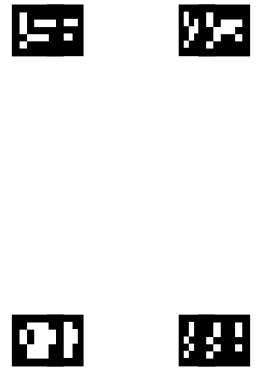
\includegraphics[scale=0.5]{ar_board_01}%
			\includesvgnew[1]{images/ar_board_01_dim}%
%		}
%		\endgroup
	}
	\hspace{-10mm}
	\subfigure[Markerfeld 2]{
%		\begingroup\fboxsep=0pt\fboxrule=1pt
%		\fbox{%
%			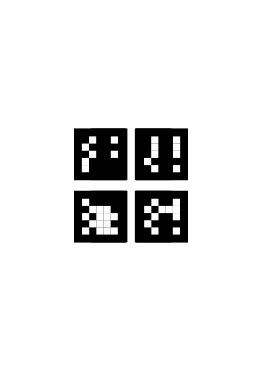
\includegraphics[scale=0.5]{ar_board_02}%
			\includesvgnew[1]{images/ar_board_02_dim}%				
%		}
%		\endgroup
	}
	\hspace{-23mm}
	\caption{Markerfelder zur Validierung der Systempose}
	\label{fig.armarker}
	\end{center}
	\vspace*{-2mm}
\end{figure}

% über $k$ Messungen aus den jeweiligen Einzeldifferenzen $r_i$ der Freiheitsgrade der Posen bestimmt:

%\begin{equation}
%\mathrm{QM} = \sqrt{\frac{1}{k} \cdot \sum_{i=1}^kr_i^2}
%\end{equation}
%
%\nomenclature[l]{$n$}{Anzahl, allgemein}
%\nomenclature[l]{$k$}{Anzahl an Messungen}
%\nomenclature[a]{QM}{Quadratisches Mittel}
%\nomenclature[l]{$r_i$}{$i$-ter Differenzwert}


\section{Globale Lokalisation}
Die globale Lokalisation bildet die Basis der Lagebestimmung des \kps{s}. Im folgenden werden das RCM und das EPM verglichen und auf ihre Eignung als globales Lokalisationsverfahren für das \kps{} geprüft. Neben der möglichst exakten Annäherung ist dabei auch eine approximative Bestimmung der Systempose von Bedeutung. Wird die Pose innerhalb eines Grenzbereiches angenähert, kann die verbleibende Abweichung durch anschließende Optimierungsschritte verringert werden. Im Falle einer fehlerhaften initialen Lokalisation kann jedoch trotz lokaler Optimierung nicht von einer Verringerung der Abweichung zur wahren Pose ausgegangen werden. Als zusätzliches Bewertungskriterium der globalen Lokalisation wird deshalb im Folgenden neben der Abweichung zur realen Pose auch die Erfolgsquote der Approximation erfasst. Als drittes Vergleichskriterium wird die für den Lokalisationsvorgang benötigte Rechenzeit ausgewertet.\\

%Dabei ist besonders eine approximative Bestimmung der Systempose von Bedeutung. Die Bestimmung einer möglichst exakten Annäherung der Pose ist zwar prinzipiell ebenso Ziel der globalen Lokalisation, kann jedoch bei korrekter initialer Approximation auch durch anschließende Optimierungsschritte erreicht werden. Im Falle einer fehlerhaften initialen Lokalisation kann trotz einer lokalen Optimierung nicht von einer Verringerung der Abweichung zur wahren Pose ausgegangen werden. Als zusätzliches Bewertungskriterium der globale Lokalisation wird deshalb im Folgenden neben der Abweichung zur realen Pose auch die Erfolgswahrscheinlichkeit der Approximation erfasst.\\

Um die wahre Pose des \kps{s} zu bestimmen wird das Markerfeld innerhalb der realen Umgebung auf einer ebenen Fläche befestigt. Der Abgleich zwischen der daraus bestimmten Pose und der durch die Lokalisation ermittelten Pose ist dabei nur möglich, wenn die Pose des Markerfeldes auch in der Modellumgebung bekannt ist. Dies kann entweder durch Anbringung der Markerfelder vor der Kartierung oder durch Definition der Markerpose anhand eindeutiger Landmarken der Umgebung erreicht werden.\\

Die Bestimmung der Referenzpose kann nun durch Erfassung des Markerfeldes mit der Kamera des Systems erfolgen. Dazu wird das \kps{} in einer Pose fixiert und die Transformation $\tmat{MF}{K}$ zwischen dem Markerfeld und der Kamera des \kps{s} bestimmt. Die Kameraperspektive mit Blick auf das Markerfeld zeigt \abb{fig.loclimits} (a). Durch die vorhandene Verknüpfung zwischen der realen und der Modellumgebung ist die Transformation $\tmat{M}{MF}$ zwischen den Koordinaten der Karte und dem Markerfeld beschrieben. Ebenso bekannt ist die statische Transformation $\tmat{K}{KPS}$ zwischen der Kamera und dem Basis-Koordinatensystem des \kps{s}. Es lässt sich somit die Transformation zwischen \kps{} und Karte bestimmen zu:
%
%
\begin{equation}
\tmat{M}{KPS} = \tmat{M}{MF} \cdot \tmat{MF}{K} \cdot \tmat{K}{KPS} \; \text{.}
\end{equation}

Aus der fixierten Pose wird anschließend die globale Lokalisation durchgeführt. Für beide Modelle werden insgesamt $k=20.000$ Partikel zufällig in der Karte verteilt. Die jeweils ermittelte Pose mit der höchsten Wahrscheinlichkeit wird anschließen mit der Referenzpose verglichen. Dazu wird das QM der Fehler bezüglich der translatorischen ($\Delta X$, $\Delta Y$, $\Delta Z$) und rotatorischen ($\Delta \Psi$, $\Delta \Theta$, $\Delta \Phi$) Freiheitsgrade des Systems bestimmt.\\

\nomenclature[l]{$\Delta X$}{Fehler in der bestimmten Pose bezüglich der $x$-Achse}
\nomenclature[l]{$\Delta Y$}{Fehler in der bestimmten Pose bezüglich der $y$-Achse}
\nomenclature[l]{$\Delta Z$}{Fehler in der bestimmten Pose bezüglich der $z$-Achse}
\nomenclature[g]{$\Delta \Phi$}{Fehler in der bestimmten Pose bezüglich des Gier-Winkels}
\nomenclature[g]{$\Delta \Theta$}{Fehler in der bestimmten Pose bezüglich des Nick-Winkels}
\nomenclature[g]{$\Delta \Psi$}{Fehler in der bestimmten Pose bezüglich des Roll-Winkels}


In der Fehlerbetrachtung sollen nur die ermittelten Posen berücksichtigt werden, welche eine Annäherung an die tatsächliche Pose innerhalb bestimmter Grenzen darstellen. Außerhalb dieses Bereiches wird von einer fehlerhaften Lokalisation ausgegangen. Um die erfolgreiche Approximation der Pose zu bewerten wird wie in \abb{fig.loclimits} (b) dargestellt deshalb ein Grenzraum um die wahre Position des \kps{s} definiert. Die maximal zulässigen translatorischen und rotatorischen Fehler sind in \tab{thresh_glob} aufgeführt. Die Definition der Grenzwerte erfolgt orientiert an Fehlerwerten, aus welchen in der Literatur eine anschließende Optimierung der angenäherten Pose erreicht werden konnte \cite{Forster2013}.\\
%\red[Festgelegt nach \cite{Forster2013}\\]

\begin{figure}[!ht]
	\begin{center}
	\subfigure[Bilddaten der RGB-Kamera mit verwendetem Markerfeld bei der globalen Lokalisation]{
		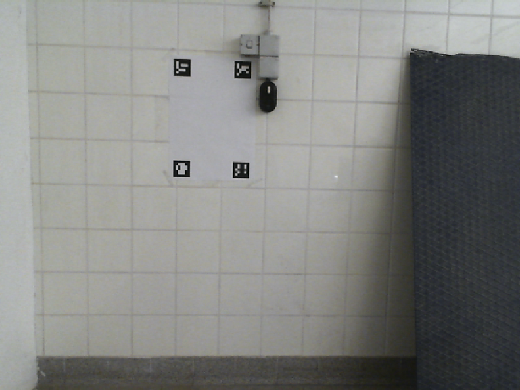
\includegraphics[scale=0.35]{glob_loc_view_03}	
	}
	\hspace{5mm}
	\subfigure[Modellansicht des Grenzbereiches der globalen Lokalisation mit korrekt angenäherter Pose (grün) und fehlerhafter Lokalisation (rot)]{
		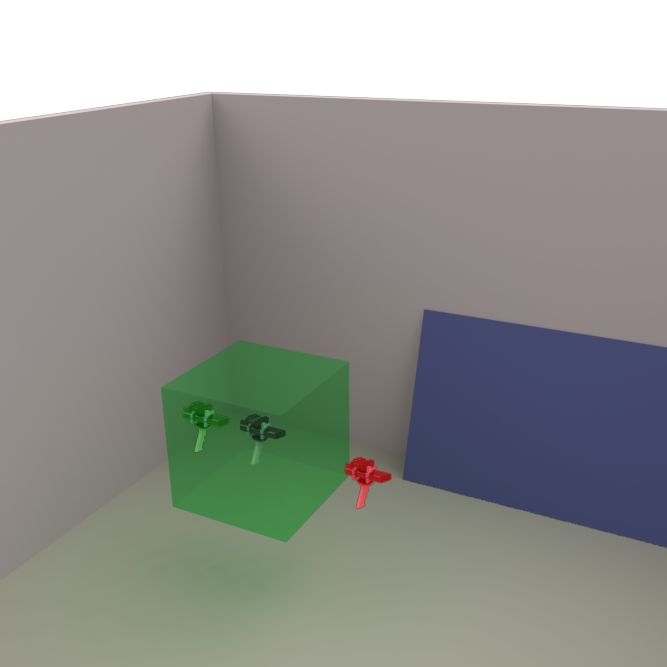
\includegraphics[scale=0.5]{glob_loc_thresh_02}
	}
	\caption{Kameraperspektive und definierter Grenzbereich der globalen Lokalisation}
		\label{fig.loclimits}
	\end{center}
\end{figure}

\prever{
%\red[Subfigure von realem Kamerabild ergänzen!\\]
}

\begin{table}[ht]
\begin{center}
\setlength{\tabcolsep}{18pt}
	\begin{tabular}[ht]{lr}
	\toprule
	Dimension		& Grenzwert 					\\ 
	\midrule 
	translatorisch  	& \SI{0,35}{\meter}			\\ \addlinespace
	rotatorisch		& \SI{7}{°}					\\ 
	\bottomrule
	\end{tabular} 
	\caption{Grenzwerte zur Bestimmung der erfolgreichen Approximation der Systempose durch die globale Lokalisation}
\label{tab.thresh_glob}
\end{center}
\end{table}

\prever{
%\red[Anzahl an Messungen ergänzen -> Aus gültigen Messungen bestimmt!?\\]
}


%\begin{table}[ht]
%\begin{center}
%	%\vspace*{-3mm}
%	\begin{tabular}[ht]{|l|r|}\hline
%		\rowcolor{Snow2}
%		Dimension		& Grenzwert 					\\ \hline
%		translatorisch  	& \SI{0,35}{\meter}			\\ \hline
%		rotatorisch		& \SI{7}{°}					\\ \hline
%	\end{tabular} 
%	\caption{Grenzwerte zur Bestimmung der erfolgreichen Approximation der Systempose durch die globale Lokalisation}
%\label{tab.thresh_glob}
%\end{center}
%\end{table}
%\vspace{3mm}

Die Erfolgsquote der Annäherung der wahren Systempose berechnet sich aus dem Quotienten der fehlgeschlagenen und insgesamt durchgeführten Lokalisationen. Als fehlgeschlagen werden dabei alle Lokalisationen betrachtet, bei welchen einer der definierten Grenzwerte überschritten wurde. Um die spätere Auswertung der Fehlerwerte der Lokalisation auf Basis hinreichend vieler Messungen zu ermöglichen, wurde die erforderliche Anzahl gültiger Messungen auf $n=12$ festgelegt. Für beide Modelle erfolgte daher eine Durchführung der Messungen, bis diese Anzahl erreicht war. Die Ergebnisse sind zusammen mit der für die globale Lokalisation durchschnittlich benötigten Rechenzeit $\bar{t}$ in \tab{approx_time} aufgeführt.\\

\begin{table}[ht]
\begin{center}
\setlength{\tabcolsep}{18pt}
	\begin{tabular}[ht]{lrrr}
	\toprule
		Modell			& Messungen 	& Erfolgsquote [$\%$]	&	Rechenzeit $\bar{t}$	 [\SI{}{\second}]	\\
		\midrule 
		Raycasting		& \SI{22}{}	& \SI{54,54}{}					&	\SI{540,69}{}			\\ \addlinespace
		Endpoint			& \SI{16}{}	& \SI{75}{}						&	\SI{55,66}{}			\\ 
		\bottomrule
	\end{tabular} 
\caption{Ermittelte Erfolgsquote und benötigte Rechenzeit der globalen Lokalisation}
\label{tab.approx_time}
\end{center}
\end{table}%

In der benötigten Rechenzeit zeigt sich deutlich der erwartete höhere Rechenaufwand bei der Verwendung des RCM. Sie beträgt nahezu das zehnfache der für das EPM benötigten Zeit. Die berechnete Erfolgsquote hingegen bestätigt nicht die durch den Rechenaufwand erwartete Genauigkeit des Modells. Nur etwa die Hälfte der Lokalisationsvorgänge des RCM wurde nach den definierten Kriterien als erfolgreich gewertet. Das EPM hingegen schaffte es in drei Viertel der Messungen, die Systempose korrekt zu approximieren.\\

%\red[Erfolgsquote interpretieren\\]
%
%Wie aus \tab{approx_time} darüber hinaus ersichtlich wird, beträgt die benötigte Rechenzeit des \red[Raycasting]-Modells fast das \SI{10}{}-fache der vom \red[Endpoint]-Model benötigten Zeit. 
%\red[Zeit der Lokalisation auswerten\\]

Da die Erfolgsquote allein kein ausreichendes Maß darstellt, um die Präzision der Annäherung zu bewerten, wird das QM der Differenzen zwischen tatsächlicher und angenäherter Pose bestimmt. Wie bereits beschrieben wurden für jedes Modell $n=12$ gültige Messungen ausgewertet. Die Ergebnisse sind in \abb{fig.glob_loc} in Abhängigkeit der verwendeten Modelle aufgeführt.

%Auch die globale Lokalisation wird durchgeführt während sich das \kps{} in der fixierten Pose befindet. Für beide Modelle werden insgesamt $n=20.000$ Partikel zufällig in der Karte verteilt. Die jeweils ermittelte Pose mit der höchsten Wahrscheinlichkeit wird anschließen mit der Referenzposition verglichen. Das quadratische Mittel der Fehler aus jeweils \red[$n$] Messungen ist bezüglich der translatorischen ($\Delta X$, $\Delta Y$, $\Delta Z$) und rotatorischen ($\Delta \Psi$, $\Delta \Theta$, $\Delta \Phi$) Freiheitsgrade des Systems sind in \abb{fig.glob_loc} in Abhängigkeit des verwendeten Modells aufgeführt.\\

\prever{
%\red[\abb{fig.error_glob_trans} zeigt den Vergleich der durch die beiden Modelle erzielten Fehlerwerte.\\]
%\red[Versuchsparameter, Partikelzahl etc.]
}

\begin{figure}[!ht]
\begin{center}
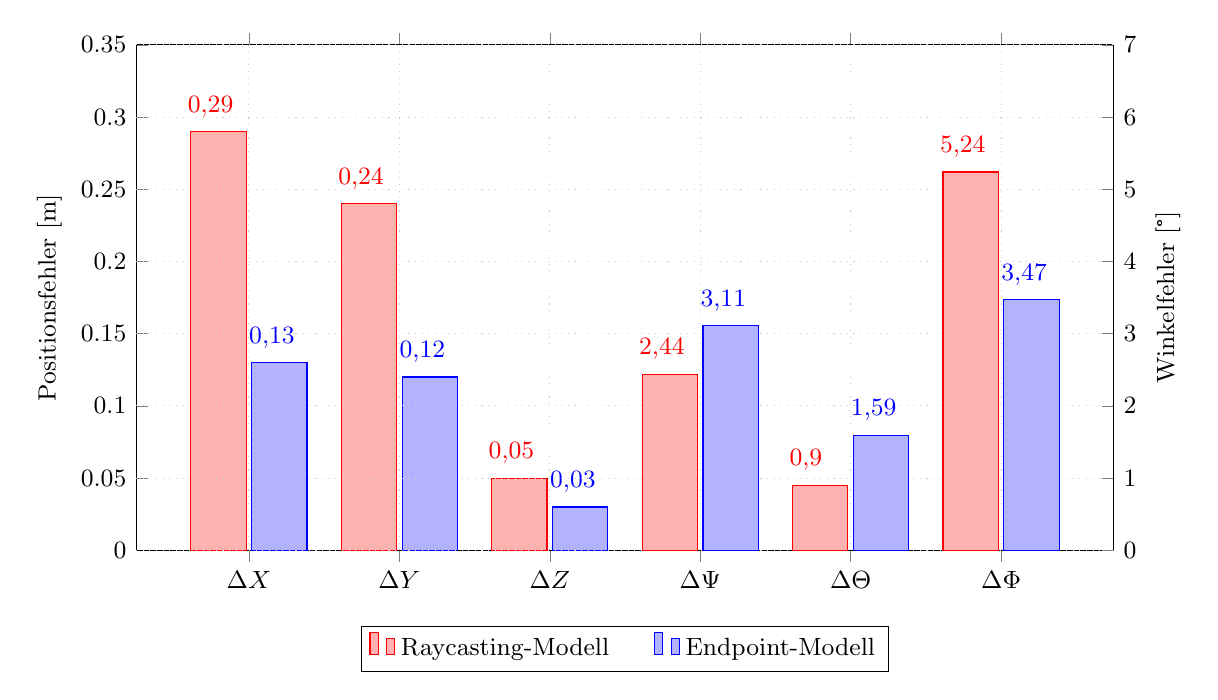
\begin{tikzpicture}
\tikzstyle{every node}=[font=\small]
\begin{axis}[
	ybar,
	ymax=0.35,
	ymin=0,
	bar width=20pt,
	scaled y ticks = false,
	y tick label style={/pgf/number format/fixed},
%	enlarge y limits={0.4,upper},
	enlarge x limits=0.15,
	legend style={at={(0.5,-0.15)},
	legend style={/tikz/every even column/.append style={column sep=0.5cm}},
	anchor=north,legend columns=-1},
	ylabel={Positionsfehler \lbrack m\rbrack},
%	symbolic x coords={\Delta,y,z},
	xtick={1,2,3,4,5,6},
	xticklabels={$\Delta X$, $\Delta Y$, $\Delta Z$, $\Delta \Psi$, $\Delta \Theta$, $\Delta \Phi$},
%	xtick=data,
	every node near coord/.style={/pgf/number format/fixed,/pgf/number format/use comma, anchor=west},
	nodes near coords,
	nodes near coords align={vertical},
	width=14cm,
	height=8cm,
	grid=major,
    	grid style={dotted,lightgray!80!white},
    	scaled y ticks = false,
]
\addplot[
	every node near coord/.append style={xshift=-0.9cm},
	nodes near coords=\raisebox{0.7cm}{\pgfmathprintnumber\pgfplotspointmeta},
	color=red,
	fill=red!30!white,
	bar shift=-11pt,
] coordinates {(1,0.29) (2,0.24) (3,0.05)};
\addplot[
	every node near coord/.append style={xshift=-0.12cm},
	nodes near coords=\raisebox{0.7cm}{\pgfmathprintnumber\pgfplotspointmeta},
	color=blue,
	fill=blue!30!white,
	bar shift=11pt,	
] coordinates {(1,0.13) (2,0.12) (3,0.03)};
\addplot[fill opacity=0.0,draw=none,] coordinates {(4,0) (5,0) (6,0)};	%dummy
\legend{Raycasting-Modell,Endpoint-Modell}
\end{axis}

\begin{axis}[
%	scale only axis,
	ybar,
	ymax=7,
	ymin=0,
	bar width=20pt,
%	enlarge y limits={0.4,upper},
	enlarge x limits=0.15,
	legend style={at={(0.5,-0.15)},
	anchor=north,legend columns=-1},
	axis y line*=right,
	axis x line=none,
	ylabel={Winkelfehler \lbrack °\rbrack},
%	symbolic x coords={\Delta,y,z},
	xtick={1,2,3,4,5,6},
	xticklabels={$\Delta X$, $\Delta Y$, $\Delta Z$, $\Delta \Psi$, $\Delta \Theta$, $\Delta \Phi$},
%	xtick=data,
%	bar shift=0pt,
	every node near coord/.style={/pgf/number format/fixed,/pgf/number format/use comma, anchor=west},
	nodes near coords,
	nodes near coords align={vertical},
	width=14cm,
	height=8cm,
	grid=major,
    	grid style={dotted,lightgray!80!white},
    	scaled y ticks = false,
]
\addplot[fill opacity=0.0,draw=none,] coordinates {(1,0) (2,0) (3,0)};	%dummy
\addplot[
	every node near coord/.append style={xshift=-0.9cm},
	nodes near coords=\raisebox{0.7cm}{\pgfmathprintnumber\pgfplotspointmeta},
	color=red,
	fill=red!30!white,
	bar shift=-11pt,	
] coordinates {(4,2.44) (5,0.90) (6,5.24)};
\addplot[
	every node near coord/.append style={xshift=-0.12cm},
	nodes near coords=\raisebox{0.7cm}{\pgfmathprintnumber\pgfplotspointmeta},
	color=blue,
	fill=blue!30!white,
	bar shift=11pt,	
] coordinates {(4,3.11) (5,1.59) (6,3.47)};
\end{axis}
\end{tikzpicture}
\end{center}

%\begin{center}
%\begin{tikzpicture}[trim axis left, trim axis right]
%\begin{axis}[
%	ybar,
%	ymax=0.4,
%	ymin=0,
%	bar width=30pt,
%	enlarge x limits=0.4,
%	legend style={at={(0.5,-0.15)},
%	anchor=north,legend columns=-1},
%	ylabel={Positionsfehler \lbrack m\rbrack},
%%	symbolic x coords={\Delta,y,z},
%	xticklabels={$\Delta X$, $\Delta Y$, $\Delta Z$},
%	xtick=data,
%	every node near coord/.style={/pgf/number format/fixed, anchor=west},
%	nodes near coords,
%	nodes near coords align={vertical},
%	width=14cm,
%	height=8cm,
%	grid=major,
%    	grid style={dotted,lightgray!80!white},
%    	scaled y ticks = false,
%]
%\addplot[
%	every node near coord/.append style={xshift=-1.1cm},
%	nodes near coords=\raisebox{0.7cm}{\pgfmathprintnumber\pgfplotspointmeta},
%	color=red,
%	fill=red!30!white
%] coordinates {(-1,0.3105647208) (0,0.3388888731) (1,0.0473358078)};
%\addplot[
%	every node near coord/.append style={xshift=0.0cm},
%	nodes near coords=\raisebox{0.7cm}{\pgfmathprintnumber\pgfplotspointmeta},
%	color=blue,
%	fill=blue!30!white
%] coordinates {(-1,0.1315834135) (0,0.1248760865) (1,0.0209899568)};
%\legend{Raycasting,Endpoint}
%\end{axis}
%\label{fig.error_glob_trans}
%\end{tikzpicture}
%\end{center}
%
%\red[Winkelfehler Vergleich:\\]
%
%\begin{center}
%\begin{tikzpicture}[trim axis left, trim axis right]
%\begin{axis}[
%	ybar,
%	ymax=10,
%	ymin=0,
%	bar width=30pt,
%%	enlarge y limits={0.4,upper},
%	enlarge x limits=0.4,
%	legend style={at={(0.5,-0.15)},
%	anchor=north,legend columns=-1},
%	ylabel={Winkelfehler \lbrack °\rbrack},
%%	symbolic x coords={\Delta,y,z},
%	xticklabels={$\Delta \Psi$, $\Delta \Theta$, $\Delta \Phi$},
%	xtick=data,
%	every node near coord/.style={/pgf/number format/fixed, anchor=west},
%	nodes near coords,
%	nodes near coords align={vertical},
%	width=14cm,
%	height=8cm,
%	grid=major,
%    	grid style={dotted,lightgray!80!white},
%    	scaled y ticks = false,
%]
%\addplot[
%	every node near coord/.append style={xshift=-1.1cm},
%	nodes near coords=\raisebox{0.7cm}{\pgfmathprintnumber\pgfplotspointmeta},
%	color=red,
%	fill=red!30!white
%] coordinates {(-1,2.4445637073) (0,0.9069805767) (1,8.4545773848)};
%\addplot[
%	every node near coord/.append style={xshift=0.0cm},
%	nodes near coords=\raisebox{0.7cm}{\pgfmathprintnumber\pgfplotspointmeta},
%	color=blue,
%	fill=blue!30!white
%] coordinates {(-1,3.1694824628) (0,1.6633422885) (1,4.2398218425)};
%\legend{Raycasting,Endpoint}
%\end{axis}
%\label{fig.error_glob_rot}
%\end{tikzpicture}
%\end{center}


%\begin{figure}[!ht]
%	\begin{center}
%	\subfigure[1. Formparameter (Fokus-Modell)]{
%		\begin{tikzpicture}[scale=0.6, baseline]
%            \begin{axis}[ybar]
%                \addplot+ coordinates {
%                    (1,2)
%                };
%            \end{axis}
%        \end{tikzpicture}
%	}
%	\hspace{2mm}
%	\subfigure[1. Formparameter (Post-Fokus-Modell)]{
%		\begin{tikzpicture}[scale=0.6, baseline]
%            \begin{axis}[ybar]
%                \addplot+ coordinates {
%                    (1,2)
%                };
%            \end{axis}
%        \end{tikzpicture}
%	}\\
%	\caption{Variation der ersten beiden Formparameter um $\pm 3 \sqrt{\lambda_i}$}
%	\label{fig.reference_building_shape_visualization}
%	\end{center}
%	\vspace*{-8mm}
%\end{figure}
\caption{Quadratisches Mittel der Fehlerwerte in der globalen Lokalisation}
\label{fig.glob_loc}
\end{figure}

\vspace{5mm}

\prever{
%\red[Abweichungen zwischen den IMU Daten erklären!? Messrauschen?\\]
}

Die bei der Lokalisation eingesetzte \textit{Octomap} wurde mit einer Auflösung von \SI{0,02}{\meter} aus der vermessenen Umgebung generiert. Der Rückprojektionsfehler der Kalibrierung der IR-Kamera beträgt \SI{0,25}{Pixel} und führt zu Positionsungenauigkeiten in der aufgenommenen Punktwolke. Die Kalibrierung der RGB-Kamera ergab einen Rückprojektionsfehler von \SI{0,23}{Pixel}, welcher sich auf die Genauigkeit der bestimmten Referenzpose des Markerfeldes auswirkt. Diese Unsicherheiten sind bei der Bewertung der Lokalisationsgüte zu berücksichtigen.\\

%eine Unsicherheit in der bestimmten Pose des Markerfeldes von etwa \SI{0,05}{\meter} angenommen werden muss.
%bei einem Abstand von \SI{0.5}{\meter} zum Markerfeld ein
Aufgrund der Programmstruktur ist die Vorgabe eines Bereiches zur Verteilung der Partikel bezüglich der Höhe ($z$-Achse des $\ks{M}$) erforderlich. Da das handgeführte \kps{} zu Beginn der Anwendung leicht in einer definierten Höhe gehalten werden kann, wurde dieser Grenzbereich mit einer Toleranz von $\pm$ \SI{0,1}{\meter} zur tatsächlichen Pose definiert. Die Fehlerwerte bezüglich $\Delta Z$ können aufgrund dieser Vorgabe nicht über der gewählten Toleranz liegen. Darüber hinaus verwendet die globale Lokalisation die Daten der IMU um die Orientierung bezüglich des Roll- ($\Psi$) und Nick-Winkels ($\Theta$) zu bestimmen. Bezüglich dieser drei Freiheitsgrade sind die Fehlerwerte damit nicht abhängig vom verwendeten Modell, wodurch sich die geringeren Differenzen zwischen den Modellen in diesen Bereichen erklären.\\

Für die modellabhängigen Fehlerwerte zeigen sich zwischen dem RCM und dem EPM jedoch deutliche Unterschiede in der Genauigkeit der ermittelten Pose. Die translatorischen Fehlerwerte betragen für das RCM mehr als das Doppelte der bei Einsatz des EPM verbleibenden Fehler. Auch in der Bestimmung des Gier-Winkels $\Phi$ liegt der Fehlerwert des RCM deutlich über dem des EPM. Die berechnete Erfolgsquote zeigte bereits, dass das RCM die Systempose im betrachteten Anwendungsfall mit geringerer Wahrscheinlichkeit annähert. Aus der Betrachtung der Fehlerwerte ergibt sich, dass die korrekt angenäherten Posen im Vergleich zum EPM darüber hinaus größere Ungenauigkeiten aufweisen.\\

Eine mögliche Ursache für die ungenauere Bestimmung der Systempose durch das RCM liegt in der größeren Toleranz des EPM gegenüber kleineren Abweichungen beim Abgleich zwischen Modell und Messwerten. Als Beispiel wird ein Partikel betrachtet, für welches die Messwerte einige Zentimeter in ein Hindernis hinein abgebildet werden. Durch Nichtbeachtung des Strahlenverlaufs unterscheidet sich die Bewertung durch das EPM in diesem Fall nicht von der Bewertung eines Partikels, für welches die Messwerte direkt mit der Außenfläche der Wand abgeglichen werden. Das RCM liefert durch den Abgleich entlang des Sensorstrahls für diese beiden Partikel jedoch deutlich unterschiedliche Fehlerwerte, weshalb das Partikel unter Umständen verworfen wird. Durch Verwendung einer größeren Varianz innerhalb des Sensormodells kann dieser Tatsache zwar entgegengewirkt werden, die Ungenauigkeit in der bestimmten Pose würde sich dadurch jedoch vergrößern.\\

Anzumerken ist, dass aufgrund der Funktionsweise eines Partikelfilters durch Erhöhung der Partikelanzahl das Raster und damit die Auflösung der betrachteten Posen nahezu infinitesimal verfeinert werden kann. Die durchgeführte Fehlerbetrachtung dient daher insbesondere als Vergleich der beiden Modelle. Die höhere Genauigkeit des EPM in der Approximation zeigt zusammen mit der größeren Erfolgswahrscheinlichkeit und der deutlich geringeren Rechenzeit, dass es für den vorliegenden Anwendungsfall gegenüber dem RCM bevorzugt werden sollte. Die Ungenauigkeiten aufgrund der Funktionsweise des EPM treten in geradlinigen Umgebungen mit geringer Komplexität in den Hintergrund. Da diese Arbeit insbesondere derartige Umgebungen betrachtet, ist das EPM besser als globales Lokalisationsverfahren für diesen Anwendungsfall geeignet als das RCM.

\prever{
%\red[Tiefenauflösung von Distanz abhängig \cite{Khoshelham2012}]
}
%Partikelfilter, deshalb immer Verbesserung theoretisch möglich, bei gleichen Prozessparametern soll jedoch vergleichbarkeit gewährleistet sein. Ziel ist anwendugnsfähiges Modell einzusetzen


%\red[Ergebnisse beschreiben und interpretieren\\]

%\red[Definition, welche als erfolgreich gelten müsste eigentlich vorher schon kommen um daraus die Fehlerwerte zu berechnen!\\]



%\red[Fazit daraus ableiten, welches besser geeignet ist? oder erst im Fazit/Zusammenfassung?\\]


%\red[Quadratischer Mittelwert QMW statt Root Mean Square RMS überall aktualisieren\\]


%\red[Relokalisation bei globaler Lokalisation beschreiben. Besser später als Ergänzung um die lokale Lokalisation zu korrigieren!\\]

\section{Lokale Lokalisation}%Tracking/Kontinuierliche Lokalisation}
Die Genauigkeit der lokalen Lokalisation wird gesondert von der durch die globale Lokalisation bestimmten Pose betrachtet. Dazu wird ebenfalls das für die Untersuchung der globalen Lokalisation verwendete Markerfeld genutzt. Die Referenzpose des Systems kann darüber bestimmt und als Initialisierung der Lokalisation verwendet werden. Zu Beginn der Messungen liegen damit keine Abweichungen zwischen der durch die Lokalisation bestimmten und der über das Markerfeld ermittelten Pose vor.\\

Zur Bewertung der kontinuierlichen Lokalisation werden translatorische und rotatorische Veränderungen der Systempose vorgenommen. Um eine Beeinflussung der Bewegungen untereinander zu vermeiden erfolgt eine separate Durchführung aller Messungen.\\

\subsection{Translatorische Bewegung}
Die translatorischen Bewegungen werden parallel ($y$-Achse des Systems) und orthogonal ($x$-Achse des Systems) zu einer definierten Betrachtungsebene durchgeführt. Die parallele Bewegung entlang der zweiten zur Ebene parallelen Achse ($z$-Achse des Systems) wird nicht gesondert betrachtet, da diese äquivalent zu der Bewegung entlang der ersten ist. \abb{fig.transmove} verdeutlicht dies und zeigt die Durchführung der Untersuchungen anhand eines modellhaften Beispiels des Versuchsaufbaus.\\

\begin{figure}[!ht]
	\begin{center}
		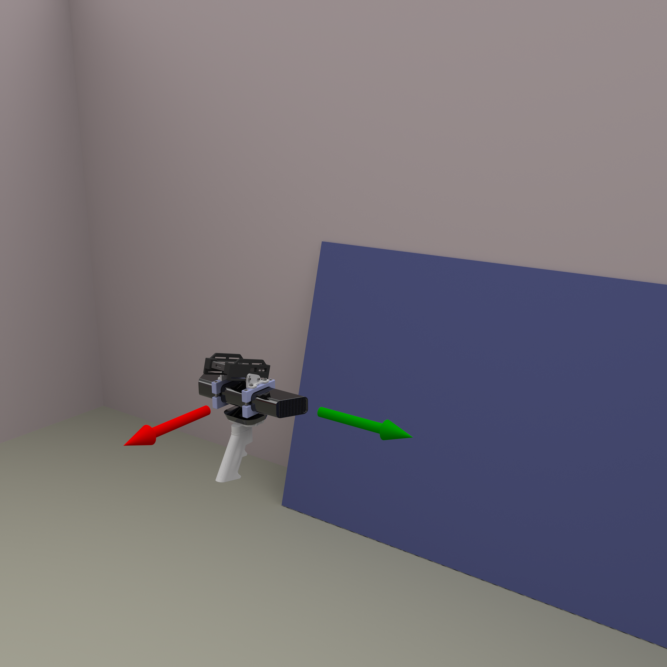
\includegraphics[scale=0.5]{loc_loc_lin}
		\caption{Aufbau zur experimentellen Auswertung der visuellen Odometrie bei translatorischer Bewegung}
		\label{fig.transmove}
	\end{center}
	%\vspace*{-8mm}
\end{figure}

Insgesamt werden für jede Achse $n=20$ Messungen ausgewertet, wobei das \kps{} bei jeder Messung um \SI{1}{\meter} translatorisch entlang der betrachteten Achse verschoben wird. Die Quadratischen Mittel der Lokalisationsfehler bei translatorischen Bewegungen parallel und orthogonal zur Betrachtungsebene sind in \abb{fig.loc_loc_trans} dargestellt.

\begin{figure}[!ht]
%---------------------------------- Translatorische Bewegung kombiniert in einem Diagramm für alle Freiheitsgrade--------------------------
\begin{center}
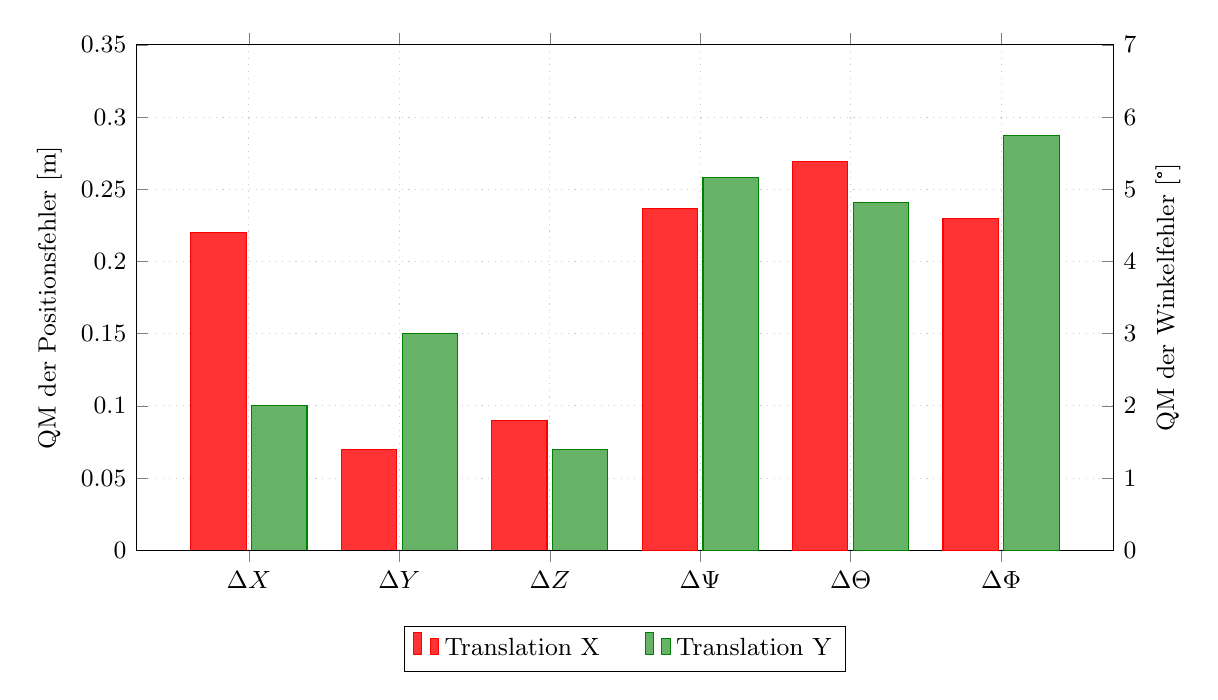
\begin{tikzpicture}
\begin{axis}[
	ybar,
	ymax=0.35,
	ymin=0,
	bar width=20pt,
	scaled y ticks = false,
	y tick label style={/pgf/number format/fixed},
%	enlarge y limits={0.4,upper},
	enlarge x limits=0.15,
	legend style={at={(0.5,-0.15)},
	legend style={/tikz/every even column/.append style={column sep=0.5cm}},
	anchor=north,legend columns=-1},
	ylabel={QM der Positionsfehler \lbrack m\rbrack},
%	symbolic x coords={\Delta,y,z},
	xtick={1,2,3,4,5,6},
	xticklabels={$\Delta X$, $\Delta Y$, $\Delta Z$, $\Delta \Psi$, $\Delta \Theta$, $\Delta \Phi$},
%	xtick=data,
%	every node near coord/.style={/pgf/number format/fixed,/pgf/number format/use comma, anchor=west},
%	nodes near coords,
%	nodes near coords align={vertical},
	width=14cm,
	height=8cm,
	grid=major,
    	grid style={dotted,lightgray!80!white},
    	scaled y ticks = false,
]
\addplot[
%	every node near coord/.append style={xshift=-0.9cm},
%	nodes near coords=\raisebox{0.7cm}{\pgfmathprintnumber\pgfplotspointmeta},
	color=Red,
	fill=Red!80!white,
	bar shift=-11pt,
] coordinates {(1,0.22) (2,0.07) (3,0.09)};
\addplot[
%	every node near coord/.append style={xshift=-0.12cm},
%	nodes near coords=\raisebox{0.7cm}{\pgfmathprintnumber\pgfplotspointmeta},
	color=Green,
	fill=Green!60!white,
	bar shift=11pt,	
] coordinates {(1,0.10) (2,0.15) (3,0.07)};
\addplot[fill opacity=0.0,draw=none,] coordinates {(4,0) (5,0) (6,0)};	%dummy
\legend{Translation X,Translation Y}
\end{axis}

\begin{axis}[
%	scale only axis,
	ybar,
	ymax=7,
	ymin=0,
	bar width=20pt,
%	enlarge y limits={0.4,upper},
	enlarge x limits=0.15,
	legend style={at={(0.5,-0.15)},
	anchor=north,legend columns=-1},
	axis y line*=right,
	ylabel={QM der Winkelfehler \lbrack °\rbrack},
%	symbolic x coords={\Delta,y,z},
	xtick={1,2,3,4,5,6},
	xticklabels={},
%	xtick=data,
%	bar shift=0pt,
%	every node near coord/.style={/pgf/number format/fixed,/pgf/number format/use comma, anchor=west},
%	nodes near coords,
%	nodes near coords align={vertical},
	width=14cm,
	height=8cm,
    	scaled y ticks = false,
]
\addplot[fill opacity=0.0,draw=none,] coordinates {(1,0) (2,0) (3,0)};	%dummy
\addplot[
%	every node near coord/.append style={xshift=-0.9cm},
%	nodes near coords=\raisebox{0.7cm}{\pgfmathprintnumber\pgfplotspointmeta},
	color=Red,
	fill=Red!80!white,
	bar shift=-11pt,	
] coordinates {(4,4.73) (5,5.39) (6,4.59)};
\addplot[
%	every node near coord/.append style={xshift=-0.12cm},
%	nodes near coords=\raisebox{0.7cm}{\pgfmathprintnumber\pgfplotspointmeta},
	color=Green,
	fill=Green!60!white,
	bar shift=11pt,	
] coordinates {(4,5.16) (5,4.82) (6,5.75)};
\end{axis}
\end{tikzpicture}
\end{center}

%----------------------------------------------------------------------------------------------------------
%------------------------------------------  Anfang  ------------------------------------------------------
%------------------------ Vergleich mit xyz rpy in getrennten Diagrammen ----------------------------------
%----------------------------------------------------------------------------------------------------------
%----------------------------------------------------------------------------------------------------------
%\subsection{Translatorische Bewegung}
%\begin{center}
%\begin{tikzpicture}[trim axis left, trim axis right]
%\begin{axis}[
%	ybar,
%	ymax=0.25,
%	ymin=0,
%	bar width=30pt,
%	enlarge x limits=0.4,
%	legend style={at={(0.5,-0.15)},
%	anchor=north,legend columns=-1},
%	ylabel={Positionsfehler \lbrack m\rbrack},
%%	symbolic x coords={\Delta,y,z},
%	xticklabels={$\Delta X$, $\Delta Y$, $\Delta Z$},
%	xtick=data,
%	every node near coord/.style={/pgf/number format/fixed, anchor=west},
%	nodes near coords,
%	nodes near coords align={vertical},
%	width=14cm,
%	height=8cm,
%	grid=major,
%    	grid style={dotted,lightgray!80!white},
%    	scaled y ticks = false,
%	y tick label style={/pgf/number format/fixed},
%]
%\addplot[
%	every node near coord/.append style={xshift=-1.1cm},
%	nodes near coords=\raisebox{0.7cm}{\pgfmathprintnumber\pgfplotspointmeta},
%	color=red,
%	fill=red!30!white
%] coordinates {(-1,0.0942737252) (0,0.0744944439) (1,0.2154737652)};
%\addplot[
%	every node near coord/.append style={xshift=0.0cm},
%	nodes near coords=\raisebox{0.7cm}{\pgfmathprintnumber\pgfplotspointmeta},
%	color=blue,
%	fill=blue!30!white
%] coordinates {(-1,0.0141228693) (0,0.0728502984) (1,0.0578491359)};
%\legend{Translatorsich X,Translatorisch Z}
%\end{axis}
%\label{fig.error_glob_trans}
%\end{tikzpicture}
%\end{center}
%
%\begin{center}
%\begin{tikzpicture}[trim axis left, trim axis right]
%\begin{axis}[
%	ybar,
%	ymax=8,
%	ymin=0,
%	bar width=30pt,
%%	enlarge y limits={0.4,upper},
%	enlarge x limits=0.4,
%	legend style={at={(0.5,-0.15)},
%	anchor=north,legend columns=-1},
%	ylabel={Winkelfehler \lbrack °\rbrack},
%%	symbolic x coords={\Delta,y,z},
%	xticklabels={$\Delta \Psi$, $\Delta \Theta$, $\Delta \Phi$},
%	xtick=data,
%	every node near coord/.style={/pgf/number format/fixed, anchor=west},
%	nodes near coords,
%	nodes near coords align={vertical},
%	width=14cm,
%	height=8cm,
%	grid=major,
%    	grid style={dotted,lightgray!80!white},
%    	scaled y ticks = false,
%	y tick label style={/pgf/number format/fixed},    	
%]
%\addplot[
%	every node near coord/.append style={xshift=-1.1cm},
%	nodes near coords=\raisebox{0.7cm}{\pgfmathprintnumber\pgfplotspointmeta},
%	color=red,
%	fill=red!30!white
%] coordinates {(-1,5.3910094725) (0,0.5944624236) (1,4.7266768476)};
%\addplot[
%	every node near coord/.append style={xshift=0.0cm},
%	nodes near coords=\raisebox{0.7cm}{\pgfmathprintnumber\pgfplotspointmeta},
%	color=blue,
%	fill=blue!30!white
%] coordinates {(-1,3.3292065305) (0,1.4935343647) (1,6.1138224963)};
%\legend{Translatorisch X,Translatorisch Z}
%\end{axis}
%\label{fig.error_loc_trans}
%\end{tikzpicture}
%\end{center}
%----------------------------------------------------------------------------------------------------------
%-------------------------------------------  Ende  -------------------------------------------------------
%------------------------ Vergleich mit xyz rpy in getrennten Diagrammen ----------------------------------
%----------------------------------------------------------------------------------------------------------
%----------------------------------------------------------------------------------------------------------

%----------------------------------------------------------------------------------------------------------
%------------------------------------------  Anfang  ------------------------------------------------------
%---------------- Vergleich mit xyz rpy in einem Diagramm, getrennt nach x und z --------------------------
%----------------------------------------------------------------------------------------------------------
%----------------------------------------------------------------------------------------------------------
%\subsection{Translation X}
%\begin{tikzpicture}
%\begin{axis}[
%	ybar,
%	ymax=0.3,
%	ymin=0,
%	bar width=30pt,
%	scaled y ticks = false,
%	y tick label style={/pgf/number format/fixed},
%% 	enlarge y limits={0.4,upper},
%	enlarge x limits=0.2,
%	legend style={at={(0.5,-0.15)},
%	anchor=north,legend columns=-1},
%	ylabel={Positionsfehler \lbrack m\rbrack},
%% 	symbolic x coords={\Delta,y,z},
%	xtick={1,2,3,4,5,6},
%	xticklabels={$\Delta X$, $\Delta Y$, $\Delta Z$, $\Delta \Psi$, $\Delta \Theta$, $\Delta \Phi$},
%% 	xtick=data,
%	bar shift=0pt,
%	every node near coord/.style={/pgf/number format/fixed, anchor=west},
%	nodes near coords,
%	nodes near coords align={vertical},
%	width=14cm,
%	height=8cm,
%	grid=major,
%	grid style={dotted,lightgray!80!white},
%	scaled y ticks = false,
%]
%\addplot[
%	every node near coord/.append style={xshift=-0.55cm},
%	nodes near coords=\raisebox{0.7cm}{\pgfmathprintnumber\pgfplotspointmeta},
%	color=red,
%	fill=red!30!white
%] coordinates {(1,0.0942737252) (2,0.0744944439) (3,0.2154737652)};
%\addplot[fill opacity=0.0,draw=none,] coordinates {(4,0) (5,0) (6,0)}; %dummy
%%\legend{Raycasting,Endpoint}
%\end{axis}
%
%\begin{axis}[
%% 	scale only axis,
%	ybar,
%	ymax=6,
%	ymin=0,
%	bar width=30pt,
%% 	enlarge y limits={0.4,upper},
%	enlarge x limits=0.2,
%	legend style={at={(0.5,-0.15)},
%	anchor=north,legend columns=-1},
%	axis y line*=right,
%	axis x line=none,
%	ylabel={Winkelfehler \lbrack °\rbrack},
%% 	symbolic x coords={\Delta,y,z},
%	xtick={1,2,3,4,5,6},
%	xticklabels={$\Delta X$, $\Delta Y$, $\Delta Z$, $\Delta \Psi$, $\Delta \Theta$, $\Delta \Phi$},
%% 	xtick=data,
%	bar shift=0pt,
%	every node near coord/.style={/pgf/number format/fixed, anchor=west},
%	nodes near coords,
%	nodes near coords align={vertical},
%	width=14cm,
%	height=8cm,
%	grid=major,
%	grid style={dotted,lightgray!80!white},
%	scaled y ticks = false,
%]
%\addplot[fill opacity=0.0,draw=none,] coordinates {(1,0) (2,0) (3,0)}; %dummy
%\addplot[
%	every node near coord/.append style={xshift=-0.55cm},
%	nodes near coords=\raisebox{0.7cm}{\pgfmathprintnumber\pgfplotspointmeta},
%	color=blue,
%	fill=blue!30!white,
%	% fill opacity=0.5,
%	% draw=none,
%] coordinates {(4,5.3910094725) (5,0.5944624236) (6,4.7266768476)};
%\end{axis}
%\label{fig.error_glob_trans_x}
%\end{tikzpicture}
%
%\subsection{Translation Z}
%\begin{tikzpicture}
%\begin{axis}[
%	ybar,
%	ymax=0.2,
%	ymin=0,
%	bar width=30pt,
%	scaled y ticks = false,
%	y tick label style={/pgf/number format/fixed},
%%	enlarge y limits={0.4,upper},
%	enlarge x limits=0.2,
%	legend style={at={(0.5,-0.15)},
%	anchor=north,legend columns=-1},
%	ylabel={Positionsfehler \lbrack m\rbrack},
%%	symbolic x coords={\Delta,y,z},
%	xtick={1,2,3,4,5,6},
%	xticklabels={$\Delta X$, $\Delta Y$, $\Delta Z$, $\Delta \Psi$, $\Delta \Theta$, $\Delta \Phi$},
%%	xtick=data,
%	bar shift=0pt,
%	every node near coord/.style={/pgf/number format/fixed, anchor=west},
%	nodes near coords,
%	nodes near coords align={vertical},
%	width=14cm,
%	height=8cm,
%	grid=major,
%    	grid style={dotted,lightgray!80!white},
%    	scaled y ticks = false,
%]
%\addplot[
%	every node near coord/.append style={xshift=-0.55cm},
%	nodes near coords=\raisebox{0.7cm}{\pgfmathprintnumber\pgfplotspointmeta},
%	color=red,
%	fill=red!30!white
%] coordinates {(1,0.0141228693) (2,0.0728502984) (3,0.0578491359)};
%\addplot[fill opacity=0.0,draw=none,] coordinates {(4,0) (5,0) (6,0)};	%dummy
%%\legend{Raycasting,Endpoint}
%\end{axis}
%
%\begin{axis}[
%%	scale only axis,
%	ybar,
%	ymax=8,
%	ymin=0,
%	bar width=30pt,
%%	enlarge y limits={0.4,upper},
%	enlarge x limits=0.2,
%	legend style={at={(0.5,-0.15)},
%	anchor=north,legend columns=-1},
%	axis y line*=right,
%	axis x line=none,
%	ylabel={Winkelfehler \lbrack °\rbrack},
%%	symbolic x coords={\Delta,y,z},
%	xtick={1,2,3,4,5,6},
%	xticklabels={$\Delta X$, $\Delta Y$, $\Delta Z$, $\Delta \Psi$, $\Delta \Theta$, $\Delta \Phi$},
%%	xtick=data,
%	bar shift=0pt,
%	every node near coord/.style={/pgf/number format/fixed, anchor=west},
%	nodes near coords,
%	nodes near coords align={vertical},
%	width=14cm,
%	height=8cm,
%	grid=major,
%    	grid style={dotted,lightgray!80!white},
%    	scaled y ticks = false,
%]
%\addplot[fill opacity=0.0,draw=none,] coordinates {(1,0) (2,0) (3,0)};	%dummy
%\addplot[
%	every node near coord/.append style={xshift=-0.55cm},
%	nodes near coords=\raisebox{0.7cm}{\pgfmathprintnumber\pgfplotspointmeta},
%	color=blue,
%	fill=blue!30!white,
%%	fill opacity=0.5,
%%	draw=none,
%] coordinates {(4,3.3292065305) (5,1.4935343647) (6,6.1138224963)};
%%\addplot[
%%	every node near coord/.append style={xshift=-1.1cm},
%%	nodes near coords=\raisebox{0.7cm}{\pgfmathprintnumber\pgfplotspointmeta},
%%	color=red,
%%	fill=red!30!white
%%] coordinates {(-2,0) (-1,0) (0,0) (1,2.4445637073) (2,0.9069805767) (3,8.4545773848)};
%\end{axis}
%\label{fig.error_glob_trans_x}
%\end{tikzpicture}
%----------------------------------------------------------------------------------------------------------
%-------------------------------------------  Ende  -------------------------------------------------------
%--------------------------- Vergleich mit xyz rpy in einem Diagramm --------------------------------------
%----------------------------------------------------------------------------------------------------------
%----------------------------------------------------------------------------------------------------------
\caption{Quadratisches Mittel der Fehlerwerte in der lokalen Lokalisation auf Basis der visuellen Odometrie bei translatorischer Bewegung}
\label{fig.loc_loc_trans}
\end{figure}

\vspace{5mm}

Beide Messreihen zeigen einen erhöhten Fehlerwert entlang der jeweiligen Translationsrichtung. Die Positionsfehler betragen dabei für die Bewegung parallel zur Betrachtungsebene etwa $15\%$ der gesamten translatorischen Distanz und für die Bewegung orthogonal zur Betrachtungsebene über $20\%$. Doch auch entlang der zur Translationsrichtung orthogonalen Ebene liegen die Fehlerwerte der Messungen bei bis zu $10\%$. Es ergibt sich damit ein deutlicher translatorischer Fehler in der durch die visuelle Odometrie bestimmten Pose.\\

Auffällig sind die trotz der rein translatorisch ausgeführten Bewegung hohen Fehler in den ermittelten Achswinkeln. Da sich aus den Ergebnissen kein direkter Zusammenhang bezüglich der Translationsrichtung ableiten lässt, deutet dies auf einen grundlegenden Fehler in der durch die visuelle Odometrie ermittelten Orientierung hin. Für eine vollständige Überprüfung sollen im Folgenden die Messungen der rein rotatorischen Bewegungen betrachtet werden.

%\red[Ergebnisse interpretieren\\]
%\red[TransX und TransZ innerhalb vergleichen und Diagramme aufteilen nach translatorischem Fehler und rotatorischem Fehler?\\Oder direkt alles in einem -> 2x6 Balken!?]

\subsection{Rotatorische Bewegung}
%\red[Vergleich zwischen Fovis und Fovis+IMU direkt zusammen in Diagramm aufführen? Erstmal nur Fovis würde dazu dienen, die Bewegungen untereinander zu vergleichen, aber was für Erkenntnisse erhält man daraus? Nick schlechter als Roll ; Nick durch IMU verbessert? -> Kompass sinnvoll! Dann evtl. aber ruhig auch Gierwinkelbewegung aufführen!\\]

Die Lokalisation während der Rotationsbewegungen wird zunächst allein auf Basis der visuellen Odometrie durchgeführt. Analog zur Auswertung der translatorischen Bewegungen werden lediglich die resultierenden Fehler aus den Rotationen um die Roll- und Nick-Achse ausgewertet. Die Rotation des Systems um die Gier-Achse unterscheidet sich für den Algorithmus der visuellen Odometrie nicht von der Rotation um die Nick-Achse, weshalb keine gesonderte Betrachtung durchgeführt wird. Die Versuchsdurchführung der Bewegungen zur Bewertung der rotatorischen Fehlereinflüsse zeigt \abb{fig.rotmove} anhand eines modellhaften Aufbaus.\\

%\prever{
%%\red[ypr alle aufführen oder nur roll und pitch, da yaw äquivalent zu pitch ist!? s.o.\\]
%}
\begin{figure}[!ht]
	\begin{center}
		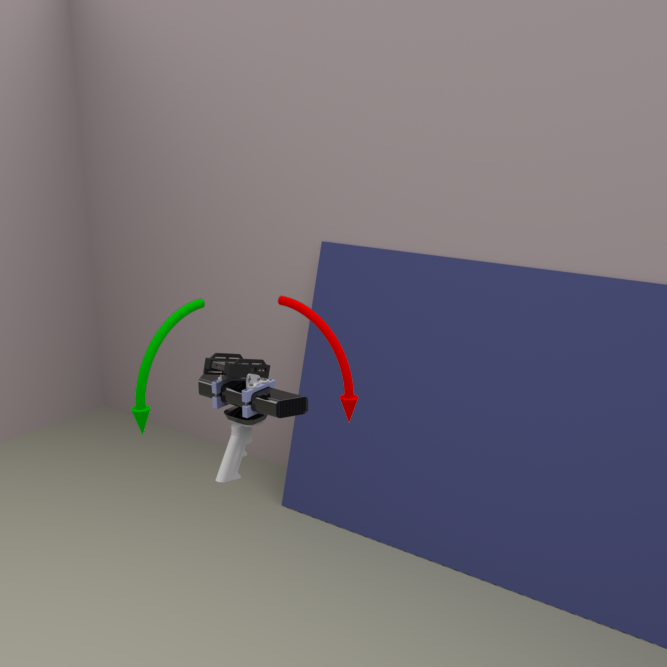
\includegraphics[scale=0.5]{loc_loc_rot_03}
		\caption{Aufbau zur experimentellen Auswertung der visuellen Odometrie bei rotatorischer Bewegung}
		\label{fig.rotmove}
	\end{center}
	%\vspace*{-5mm}
\end{figure}

%\prever{
%%\red[Bilder des Aufbaus als subfigures!?\\]
%%\red[Doch nur zwei Freiheitsgrade betrachtet!\\]
%}
%\prever{
%\subsubsection{Visuelle Odometrie}
%}
Für alle Messungen wird eine Rotation des \kps{s} von \SI{45}{°} um die betrachtete Achse ausgeführt. Die Quadratischen Mittel der in jeweils $k=20$ Messungen ermittelten Fehler zeigt \abb{fig.loc_loc_rot_fovis}.\\

\begin{figure}[!ht]
\begin{center}
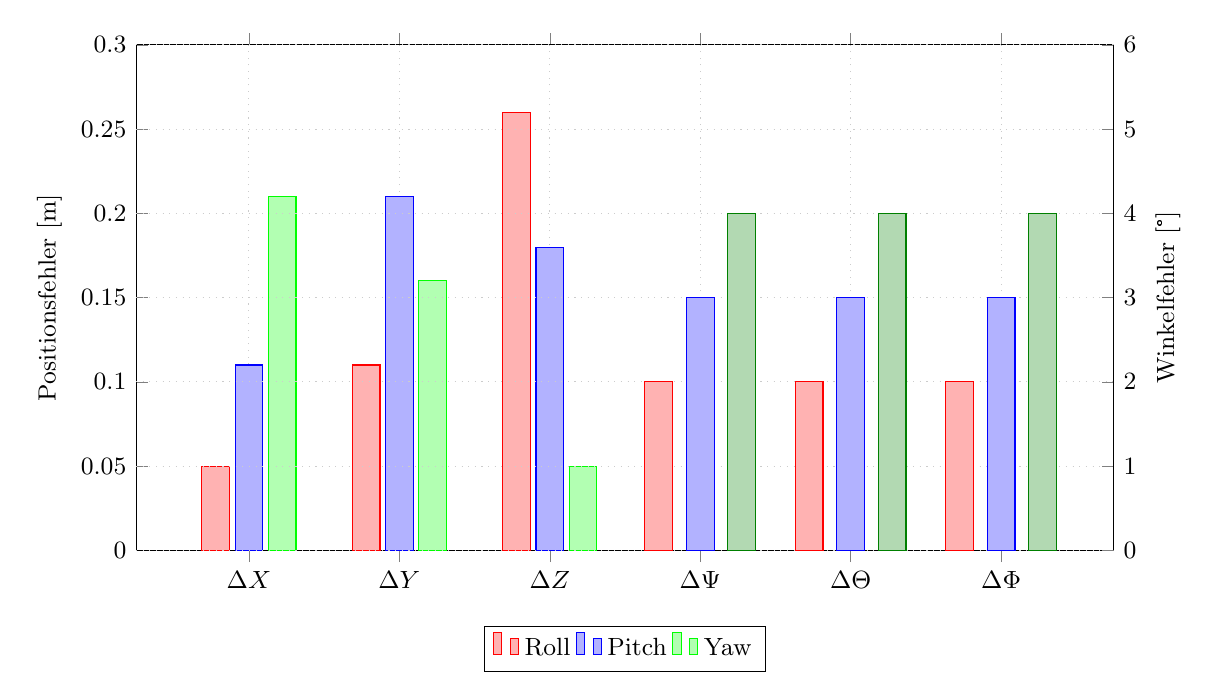
\begin{tikzpicture}
\begin{axis}[
	ybar,
	ymax=0.3,
	ymin=0,
	bar width=10pt,
	scaled y ticks = false,
	y tick label style={/pgf/number format/fixed},
%	enlarge y limits={0.4,upper},
	enlarge x limits=0.15,
	legend style={at={(0.5,-0.15)},
	anchor=north,legend columns=-1},
	ylabel={Positionsfehler \lbrack m\rbrack},
%	symbolic x coords={\Delta,y,z},
	xtick={1,2,3,4,5,6},
	xticklabels={$\Delta X$, $\Delta Y$, $\Delta Z$, $\Delta \Psi$, $\Delta \Theta$, $\Delta \Phi$},
%	xtick=data,
%	every node near coord/.style={/pgf/number format/fixed, anchor=west},
%	nodes near coords,
%	nodes near coords align={vertical},
	width=14cm,
	height=8cm,
	grid=major,
    	grid style={dotted,lightgray!80!white},
    	scaled y ticks = false,
]
\addplot[
%	every node near coord/.append style={xshift=-0.95cm},
%	nodes near coords=\raisebox{0.7cm}{\pgfmathprintnumber\pgfplotspointmeta},
	color=red,
	fill=red!30!white,
	bar shift=-12pt,
] coordinates {(1,0.05) (2,0.11) (3,0.26)};
\addplot[
%	every node near coord/.append style={xshift=-0.41cm},
%	nodes near coords=\raisebox{0.7cm}{\pgfmathprintnumber\pgfplotspointmeta},
	color=blue,
	fill=blue!30!white,
	bar shift=0pt,	
] coordinates {(1,0.11) (2,0.21) (3,0.18)};
\addplot[
%	every node near coord/.append style={xshift=0.12cm},
%	nodes near coords=\raisebox{0.7cm}{\pgfmathprintnumber\pgfplotspointmeta},
	color=green,
	fill=green!30!white,
	bar shift=12pt,	
] coordinates {(1,0.21) (2,0.16) (3,0.05)};
\addplot[fill opacity=0.0,draw=none,] coordinates {(4,0) (5,0) (6,0)};	%dummy
\legend{Roll,Pitch,Yaw}
\end{axis}

\begin{axis}[
%	scale only axis,
	ybar,
	ymax=6,
	ymin=0,
	bar width=10pt,
%	enlarge y limits={0.4,upper},
	enlarge x limits=0.15,
	legend style={at={(0.5,-0.15)},
	anchor=north,legend columns=-1},
	axis y line*=right,
	axis x line=none,
	ylabel={Winkelfehler \lbrack °\rbrack},
%	symbolic x coords={\Delta,y,z},
	xtick={1,2,3,4,5,6},
	xticklabels={$\Delta X$, $\Delta Y$, $\Delta Z$, $\Delta \Psi$, $\Delta \Theta$, $\Delta \Phi$},
%	xtick=data,
%	bar shift=0pt,
%	every node near coord/.style={/pgf/number format/fixed, anchor=west},
%	nodes near coords,
%	nodes near coords align={vertical},
	width=14cm,
	height=8cm,
	grid=major,
    	grid style={dotted,lightgray!80!white},
    	scaled y ticks = false,
]
\addplot[fill opacity=0.0,draw=none,] coordinates {(1,0) (2,0) (3,0)};	%dummy
\addplot[
%	every node near coord/.append style={xshift=-0.9cm},
%	nodes near coords=\raisebox{0.7cm}{\pgfmathprintnumber\pgfplotspointmeta},
	color=Red,
	fill=Red!30!white,
	bar shift=-15pt,	
] coordinates {(4,2) (5,2) (6,2)};
\addplot[
%	every node near coord/.append style={xshift=-0.12cm},
%	nodes near coords=\raisebox{0.7cm}{\pgfmathprintnumber\pgfplotspointmeta},
	color=Blue,
	fill=Blue!30!white,
	bar shift=0pt,	
] coordinates {(4,3) (5,3) (6,3)};
\addplot[
%	every node near coord/.append style={xshift=-0.12cm},
%	nodes near coords=\raisebox{0.7cm}{\pgfmathprintnumber\pgfplotspointmeta},
	color=Green,
	fill=Green!30!white,
	bar shift=15pt,	
] coordinates {(4,4) (5,4) (6,4)};
\end{axis}
\label{fig.loc_loc_rot_fovis}
\end{tikzpicture}
\end{center}
\caption{Quadratisches Mittel der Fehlerwerte in der lokalen Lokalisation auf Basis der visuellen Odometrie bei rotatorischer Bewegung}
\label{fig.loc_loc_rot_fovis}
\end{figure}%
%\vspace{-5mm}

%\red[Ergebnisse interpretieren\\]

Die Ergebnisse zeigen für alle Achsen einen verbleibenden translatorischen Fehler von unter $10\%$. Die Quadratischen Mittel der rotatorischen Differenzen betragen ebenfalls um $10\%$ und liegen damit nur geringfügig unter den gemessenen Winkelfehlern der translatorischen Bewegungen. Es zeigt sich damit, dass die innerhalb der vorliegenden Rahmenbedingungen über die visuelle Odometrie bestimmten Positionen und Orientierungen unabhängig von der ausgeführten Bewegung mit deutlichen Fehlern behaftet sind.\\

%\red[Allgemein stark abhängig von Features]\\
Eine Erklärung dafür könnte eine geringe Anzahl an zuverlässig ermittelten Deskriptoren innerhalb der Kamerabilder sein. Je weniger Merkmale in der Umgebung erkannt werden, desto größer wird der Einfluss fehlerhafter Detektionen auf das Resultat. Das Unterschreiten einer definierten Anzahl an detektierten Merkmalen kann darüber hinaus dazu führen, dass zwischenzeitlich keine Lokalisationsdaten ermittelt werden können. Die visuelle Odometrie basiert wie in \kapitel{locloc} beschrieben auf dem Abgleich von Merkmalen, welche sich sowohl in den aufgenommen Farb- als auch in den Tiefenwerten wiederfinden. Aus dem Anwendungsziel des \kps{s} ergibt sich insbesondere auch der Einsatz in Umgebungen mit wenigen solcher Merkmale. Auch die experimentelle Auswertung wurde deshalb in einer derartigen Umgebung durchgeführt.\\

Eine weitere Fehlerursache bezüglich der bestimmten Orientierung ergibt sich aus den Anforderungen der verwendeten Implementierung. Diese erfordert eine hohe Frequenz in der Berechnung, um Rotationen korrekt anzunähern \cite{Fovis}. Obwohl die Kinect Bilddaten mit einer Rate von \SI{30}{} Bildern pro Sekunde liefert konnten auf dem verwendeten System während der Anwendung nur etwa \SI{5}{} Bilder pro Sekunde ausgewertet werden. Dies ist zum einen auf die Komplexität der Berechnungen zur Bestimmung der visuellen Odometrie und zum anderen auf die hohe Auslastung der Rechenkapazität aufgrund der weiteren verwendeten Softwarekomponenten zurückzuführen.\\ 

%\red[-> Korrektur durch EKF möglich!?\\]
Insgesamt zeigen die Ergebnisse, dass das Verfahren der visuellen Odometrie alleine auf dem verwendeten System nicht in der Lage ist die Veränderungen der Systempose präzise zu bestimmen. Um eine Möglichkeit zur Erhöhung der Robustheit zu betrachten, werden die Untersuchungen der rotatorischen Bewegungen unter Einsatz des EKF wiederholt. Die Daten der visuellen Odometrie werden dabei mit den Orientierungs- und Beschleunigungsdaten der IMU fusioniert.

\subsection{Erweitertes Kalman-Filter}
Die Messungen werden auf gleiche Weise wie zuvor durchgeführt. Verglichen werden die Fehler in der ermittelten Systempose auf Basis der visuellen Odometrie und unter Verwendung des EKF. In \abb{fig.loc_loc_rot_ekf_roll} ist der Vergleich bezüglich der Rotation um die Roll- und in \abb{fig.loc_loc_rot_ekf_pitch} bezogen auf die Nick-Achse dargestellt.\\

%\red[Um die Fusion der Sensordaten mit den Daten der inertialen Messeinheit zu bewerten erfolgt anschließend ein Vergleich mit der Lokalisation auf Basis des Erweiterten Kalman Filters.\\]

\begin{figure}[!ht]
\begin{center}
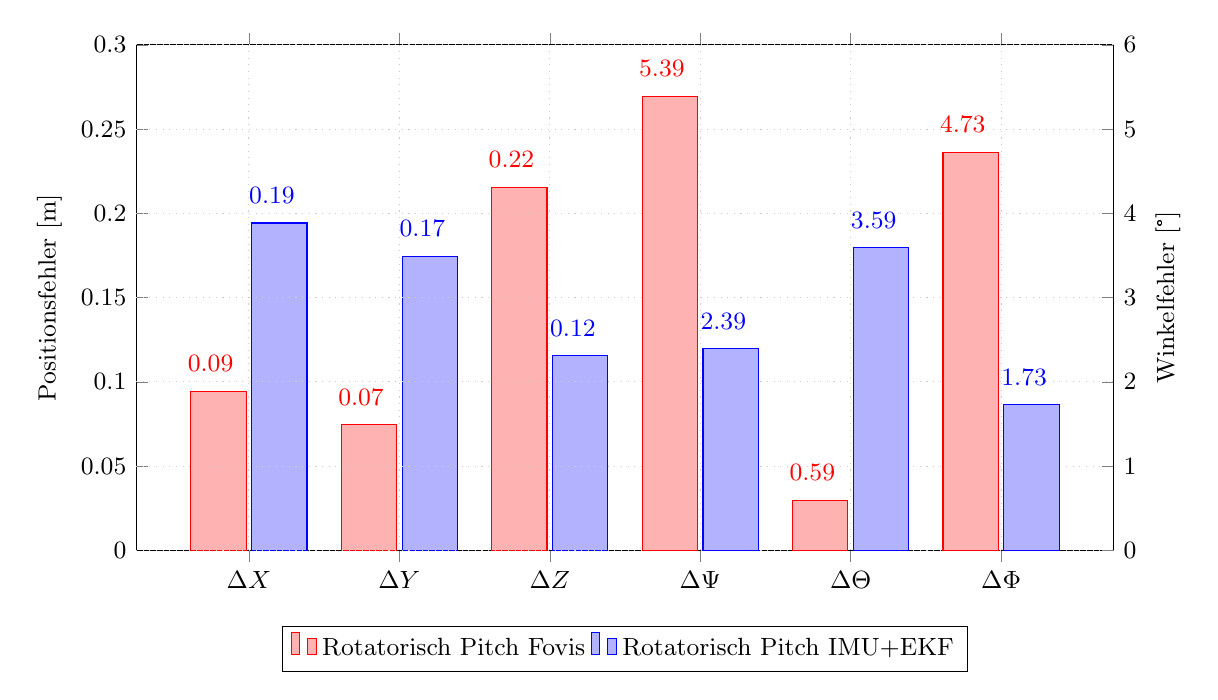
\begin{tikzpicture}
\begin{axis}[
	ybar,
	ymax=0.3,
	ymin=0,
	bar width=20pt,
	scaled y ticks = false,
	y tick label style={/pgf/number format/fixed},
%	enlarge y limits={0.4,upper},
	enlarge x limits=0.15,
	legend style={at={(0.5,-0.15)},
	anchor=north,legend columns=-1},
	ylabel={Positionsfehler \lbrack m\rbrack},
%	symbolic x coords={\Delta,y,z},
	xtick={1,2,3,4,5,6},
	xticklabels={$\Delta X$, $\Delta Y$, $\Delta Z$, $\Delta \Psi$, $\Delta \Theta$, $\Delta \Phi$},
%	xtick=data,
	every node near coord/.style={/pgf/number format/fixed, anchor=west},
	nodes near coords,
	nodes near coords align={vertical},
	width=14cm,
	height=8cm,
	grid=major,
    	grid style={dotted,lightgray!80!white},
    	scaled y ticks = false,
]
\addplot[
	every node near coord/.append style={xshift=-0.9cm},
	nodes near coords=\raisebox{0.7cm}{\pgfmathprintnumber\pgfplotspointmeta},
	color=red,
	fill=red!30!white,
	bar shift=-11pt,
] coordinates {(1,0.0942737252) (2,0.0744944439) (3,0.2154737652)};
\addplot[
	every node near coord/.append style={xshift=-0.12cm},
	nodes near coords=\raisebox{0.7cm}{\pgfmathprintnumber\pgfplotspointmeta},
	color=blue,
	fill=blue!30!white,
	bar shift=11pt,	
] coordinates {(1,0.1942737252) (2,0.1744944439) (3,0.1154737652)};
\addplot[fill opacity=0.0,draw=none,] coordinates {(4,0) (5,0) (6,0)};	%dummy
\legend{Rotatorisch Pitch Fovis,Rotatorisch Pitch IMU+EKF}
\end{axis}

\begin{axis}[
%	scale only axis,
	ybar,
	ymax=6,
	ymin=0,
	bar width=20pt,
%	enlarge y limits={0.4,upper},
	enlarge x limits=0.15,
	legend style={at={(0.5,-0.15)},
	anchor=north,legend columns=-1},
	axis y line*=right,
	axis x line=none,
	ylabel={Winkelfehler \lbrack °\rbrack},
%	symbolic x coords={\Delta,y,z},
	xtick={1,2,3,4,5,6},
	xticklabels={$\Delta X$, $\Delta Y$, $\Delta Z$, $\Delta \Psi$, $\Delta \Theta$, $\Delta \Phi$},
%	xtick=data,
%	bar shift=0pt,
	every node near coord/.style={/pgf/number format/fixed, anchor=west},
	nodes near coords,
	nodes near coords align={vertical},
	width=14cm,
	height=8cm,
	grid=major,
    	grid style={dotted,lightgray!80!white},
    	scaled y ticks = false,
]
\addplot[fill opacity=0.0,draw=none,] coordinates {(1,0) (2,0) (3,0)};	%dummy
\addplot[
	every node near coord/.append style={xshift=-0.9cm},
	nodes near coords=\raisebox{0.7cm}{\pgfmathprintnumber\pgfplotspointmeta},
	color=Red,
	fill=Red!30!white,
	bar shift=-11pt,	
] coordinates {(4,5.3910094725) (5,0.5944624236) (6,4.7266768476)};
\addplot[
	every node near coord/.append style={xshift=-0.12cm},
	nodes near coords=\raisebox{0.7cm}{\pgfmathprintnumber\pgfplotspointmeta},
	color=Blue,
	fill=Blue!30!white,
	bar shift=11pt,	
] coordinates {(4,2.3910094725) (5,3.5944624236) (6,1.7266768476)};
\end{axis}
\label{fig.loc_loc_rot_ekf_roll}
\end{tikzpicture}
\end{center}
\caption{Quadratisches Mittel der Fehlerwerte der lokalen Lokalisation bei Verwendung der visuellen Odometrie und des EKF. Durchführung einer rotatorischen Bewegung um die Roll-Achse}
\label{fig.loc_loc_rot_ekf_roll}
\end{figure}%
%\vspace{-2mm}

\begin{figure}[!ht]
\begin{center}
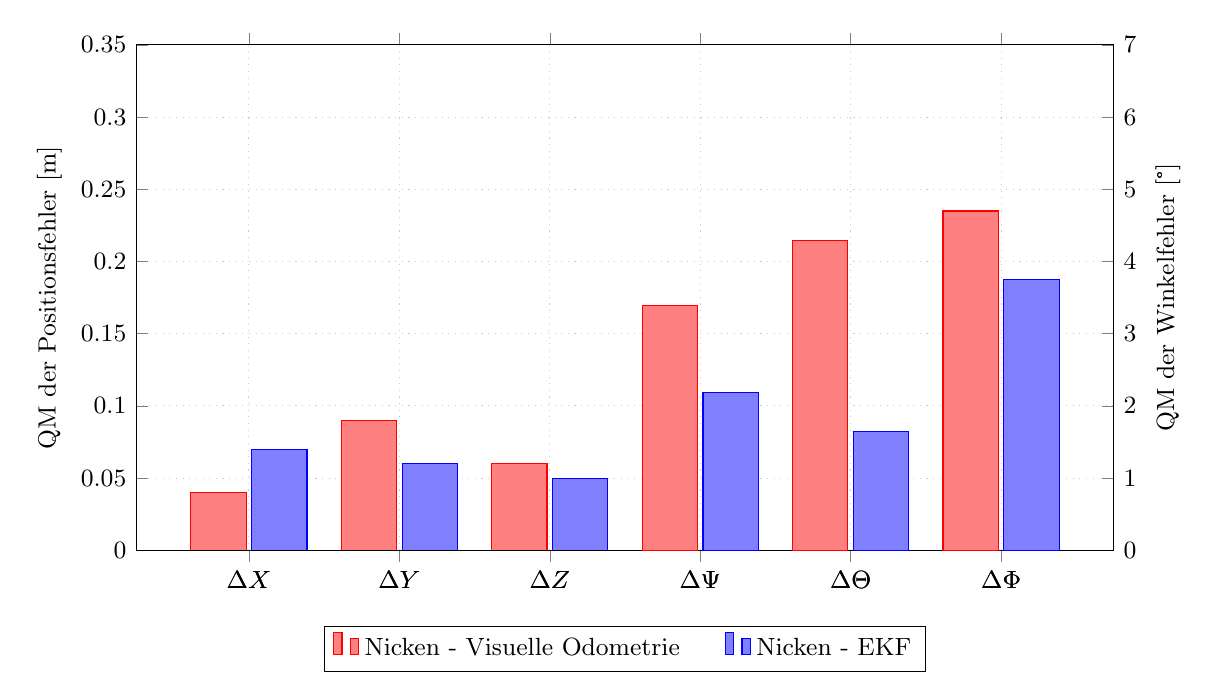
\begin{tikzpicture}
\begin{axis}[
	ybar,
	ymax=0.35,
	ymin=0,
	bar width=20pt,
	scaled y ticks = false,
	y tick label style={/pgf/number format/fixed},
%	enlarge y limits={0.4,upper},
	enlarge x limits=0.15,
	legend style={at={(0.5,-0.15)},
	legend style={/tikz/every even column/.append style={column sep=0.5cm}},
	anchor=north,legend columns=-1},
	ylabel={QM der Positionsfehler \lbrack m\rbrack},
%	symbolic x coords={\Delta,y,z},
	xtick={1,2,3,4,5,6},
	xticklabels={$\Delta X$, $\Delta Y$, $\Delta Z$, $\Delta \Psi$, $\Delta \Theta$, $\Delta \Phi$},
%	xtick=data,
%	every node near coord/.style={/pgf/number format/fixed,/pgf/number format/use comma, anchor=west},
%	nodes near coords,
%	nodes near coords align={vertical},
	width=14cm,
	height=8cm,
	grid=major,
    	grid style={dotted,lightgray!80!white},
    	scaled y ticks = false,
]
\addplot[
%	every node near coord/.append style={xshift=-0.9cm},
%	nodes near coords=\raisebox{0.7cm}{\pgfmathprintnumber\pgfplotspointmeta},
	color=red,
	fill=red!50!white,
	bar shift=-11pt,
] coordinates {(1,0.04) (2,0.09) (3,0.06)};
\addplot[
%	every node near coord/.append style={xshift=-0.12cm},
%	nodes near coords=\raisebox{0.7cm}{\pgfmathprintnumber\pgfplotspointmeta},
	color=blue,
	fill=blue!50!white,
	bar shift=11pt,	
] coordinates {(1,0.07) (2,0.06) (3,0.05)};
\addplot[fill opacity=0.0,draw=none,] coordinates {(4,0) (5,0) (6,0)};	%dummy
\legend{Nicken - Visuelle Odometrie,Nicken - EKF}
\end{axis}

\begin{axis}[
%	scale only axis,
	ybar,
	ymax=7,
	ymin=0,
	bar width=20pt,
%	enlarge y limits={0.4,upper},
	enlarge x limits=0.15,
	legend style={at={(0.5,-0.15)},
	anchor=north,legend columns=-1},
	axis y line*=right,
	ylabel={QM der Winkelfehler \lbrack °\rbrack},
%	symbolic x coords={\Delta,y,z},
	xtick={1,2,3,4,5,6},
	xticklabels={$\Delta X$, $\Delta Y$, $\Delta Z$, $\Delta \Psi$, $\Delta \Theta$, $\Delta \Phi$},
%	xtick=data,
%	bar shift=0pt,
%	every node near coord/.style={/pgf/number format/fixed,/pgf/number format/use comma, anchor=west},
%	nodes near coords,
%	nodes near coords align={vertical},
	width=14cm,
	height=8cm,
    	scaled y ticks = false,
]
\addplot[fill opacity=0.0,draw=none,] coordinates {(1,0) (2,0) (3,0)};	%dummy
\addplot[
%	every node near coord/.append style={xshift=-0.9cm},
%	nodes near coords=\raisebox{0.7cm}{\pgfmathprintnumber\pgfplotspointmeta},
	color=red,
	fill=red!50!white,
	bar shift=-11pt,	
] coordinates {(4,3.39) (5,4.29) (6,4.70)};
\addplot[
%	every node near coord/.append style={xshift=-0.12cm},
%	nodes near coords=\raisebox{0.7cm}{\pgfmathprintnumber\pgfplotspointmeta},
	color=blue,
	fill=blue!50!white,
	bar shift=11pt,	
] coordinates {(4,2.18) (5,1.64) (6,3.75)};
\end{axis}
\end{tikzpicture}
\end{center}
\caption{Quadratisches Mittel der Fehlerwerte der lokalen Lokalisation bei Verwendung der visuellen Odometrie und des EKF. Durchführung einer rotatorischen Bewegung um die Nick-Achse}
\label{fig.loc_loc_rot_ekf_pitch}
\end{figure}

%\red[Ergebnisse interpretieren\\]

In beiden Messreihen zeigen sich deutliche Auswirkungen auf die Freiheitsgrade, für welche die IMU Orientierungsdaten bereitstellt. Die Fusion der Sensorwerte führt zu einer starken Verringerung der Fehler in der Winkelbestimmung bezüglich der Roll- und Nick-Achse. Geringe Auswirkungen zeigen sich auch auf die gemessenen Fehlerwerte der weiteren Freiheitsgrade. Diese Abweichungen erklären sich aus der Approximation durch das EKF und der Verbesserung in der Bestimmung des Roll- und Nick-Winkels, wobei für die verschiedenen Freiheitsgrade sowohl Verringerungen als auch Zunahmen der Fehlerwerte zu beobachten sind. Insgesamt konnte die Genauigkeit der Lokalisation während der kontinuierlichen Bestimmung der Pose durch die Fusion der Sensordaten mittels des EKF somit für zwei der sechs Freiheitsgrade erhöht werden.\\ 

\prever{
%\red[Da das \kps{} als Starrkörper betrachtet werden kann, ergeben sich durch die \\]
}

Um die Fehlerfortpflanzung im Verlauf der lokalen Lokalisation zu verringern wurde die Implementierung der globalen Lokalisation um zusätzliche Funktionalität erweitert. Dabei wird die Ausführung einer modifizierten Variante der globalen Lokalisation ermöglicht. In einem definierten Parameterbereich werden Partikel um die aktuelle Pose gestreut, so dass das lokale Optimum neu ermittelt wird. Die verwendete Anzahl Partikel kann dabei geringer gewählt werden als bei der globalen Lokalisation, wodurch dieser Schritt mit deutlich geringerer Rechenzeit verbunden ist. Diese Funktion kann automatisch oder manuell durch den Benutzer aufgerufen werden, so dass zu definierten Zeitpunkten eine Korrektur der ermittelten Pose erzielt wird. Dabei ermöglicht die in \kapitel{chap.projection} beschriebene visuelle Rückmeldung über den aktuellen Überdeckungsfehler dem Anwender eine direkte Bewertung der korrigierten Pose.

%\red[Globale Lokalisation mit weniger Partikel als lokale Lokalisation verwenden! -> Hier aufführen? Ohne Messungen?]

\prever{
%\red[(englisch inertial measurement unit, IMU) -> IMU überall ersetzen\\]
}
%\subsection{Rotation Roll IMU+KALMAN}


%\red[Mögliche Lösungsansätze hier thematisieren?\\] 

\section{Visualisierung}
Um die lagerichtige Abbildung der visuellen Zusatzinformationen in der realen Umgebung zu ermöglichen ist über die Lokalisation hinaus auch eine hohe Genauigkeit der Projektion erforderlich. Die Interaktion des Benutzers mit der Projektion erfordert zudem eine dynamische Darstellung mit geringer Verzögerung. Im Folgenden soll deshalb im Rahmen experimenteller Untersuchungen zunächst die Projektionsgenauigkeit und abschließend die Latenzzeit der Visualisierung ermittelt werden.

\subsection{Projektionsgenauigkeit}
Die Genauigkeit der Projektion virtueller Modelldaten wird unter Verwendung einer externen Kamera analysiert. Diese wird zunächst analog zu dem in \kapitel{chap.calib} beschriebenen Vorgehen für die RGB-Kamera der Kinect kalibriert, wodurch eine objektive Betrachtung der Projektionsgenauigkeit ermöglicht wird. Der Rückprojektionsfehler der Kalibrierung der externen Kamera beträgt \SI{0,26}{Pixel}, die Kalibrierung des \kps{s} ergab einen horizontalen Projektionsfehler von $e_\ind{x} = \SI{1,57}{Pixel}$ und einen vertikalen Projektionsfehler von $e_\ind{y} = \SI{1}{Pixel}$. Für die Untersuchung wird ein Markerfeld auf einer ebenen Unterlage fixiert und im Sicht- und Projektionsfeld des \kps{s} platziert. Das Markerfeld wird mittels der RGB-Kamera der Kinect erfasst, um die Transformation des \kps{s} relativ zum Markerfeld zu bestimmen.\\

Die bekannte Transformation zwischen Kamera- und Projektorkoordinaten ermöglicht die Zuordnung der detektierten 3D-Koordinaten des Markerfeldes zu den 2D-Koordinaten des Projektorbildes. Um die Projektionsgenauigkeit zu überprüfen wird mittels des Projektors ein weiteres Markerfeld projiziert, welches bezogen auf die Projektorkoordinaten deckungsgleich mit dem realen Markerfeld ist. Dazu werden beide Markerfelder in der Modellumgebung dargestellt und überlagert. Die externe Kamera wird anschließend so positioniert, dass sie in der Lage ist das reale und das projizierte Markerfeld zu erfassen. Es ergibt sich daraus der in \abb{fig.projsetup} dargestellte Versuchsaufbau.

\begin{figure}[!ht]
	\begin{center}%
		\includesvgnew[1]{images/projection_validation_cropped_02}%
		\caption{Aufbau zur Überprüfung der Projektionsgenauigkeit}
		\label{fig.projsetup}
	\end{center}
	%\vspace*{-8mm}
\end{figure}
%\red[Projiziertes Feld: Kästchen entfernen!\\]

Durch Detektion der Markerfelder im Bild der externen Kamera können wie in \abb{fig.arprojected} dargestellt die Transformationen bezüglich der Kamera ermittelt werden. Aus dem Vergleich der Transformation zwischen den Feldern lassen sich die Abweichungen bezüglich Position und Orientierung bestimmen. Sowohl die Positionierung des \kps{s} als auch der externen Kamera wird dabei während der Untersuchungen variiert.\\

\prever{
%\red[Markerlokalisation ausführen -> schon zu Beginn!\\]
}

\begin{figure}[!ht]
	\begin{center}
		\includesvgnew[1]{images/board_eval_cropped_02}%
%		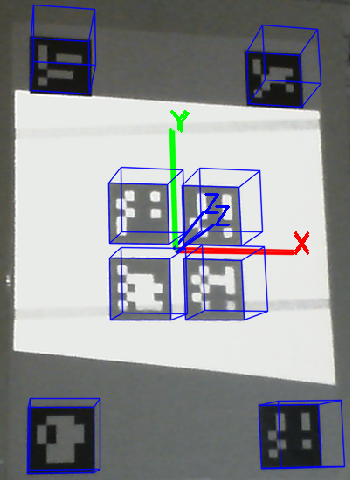
\includegraphics[scale=0.3]{board_eval_cropped}
		\caption{Detektion der Pose des realen und projizierten Markerfeldes im Bild der externen Kamera}
		\label{fig.arprojected}
	\end{center}
	%\vspace*{-8mm}
\end{figure}%

Die ermittelten Fehler der $k=6$ Messreihen mit insgesamt $n=229$ Messungen sind als Box-Whisker-Plot in \abb{fig.boxplot_proj} dargestellt. Dabei wurde die Gesamtheit der Messwerte in die Darstellung aufgenommen. Die minimalen und maximalen Messwerte werden durch die Whisker beschrieben, während die Boxen das zweite und dritte Quartil abbilden. Der Median ist als Trennlinie innerhalb der Boxen repräsentiert. Für eine bessere Übersicht orientiert sich die farbliche Abbildung der Messungen an der verwendeten RGB-Darstellung der Koordinatensysteme.

\prever{
%\red[Box Whisker Plot erklären -> Gesamte Messreihe, IQR,Median,keine Ausreisser\\]
}

\begin{figure}[!ht]
\begin{center}
\begin{tikzpicture}[trim axis left, trim axis right]
  \begin{axis}[
    	ytick={-30,-20,...,30},
    		minor y tick num=1,
    		ymax=35,
    		ymin=-35,
    		ylabel=Positionsfehler \lbrack mm\rbrack,
    		xtick={1,2,...,6},
    		x tick label style={align=center},
    		xticklabels={$\Delta X$, $\Delta Y$, $\Delta Z$, $\Delta \Psi$, $\Delta \Theta$, $\Delta \Phi$},
    		boxplot/draw direction=y,
    		width=14cm,
    		height=8cm,
    		grid=major,
    		grid style={dotted,lightgray!80!white},
    ]
    \addplot+[color=red,mark=x,
    		boxplot prepared={
      		lower whisker=-7.2937458753,
      		lower quartile=-2.2697057575,
      		median=-0.5078930408,
      		upper quartile=2.5787912309,
      		upper whisker=5.2836090326,
      		box extend=0.5,
      		draw position=1,
    		},
    ] coordinates {};
    %table[row sep=\\,y index=0] {0.0\\}; %Ausreisser
    \addplot+[color=Green,mark=x,
    		boxplot prepared={
      		lower whisker=-5.6481547653,
      		lower quartile=0.8273310959,
      		median=2.7935747058,
      		upper quartile=6.1452584341,
      		upper whisker=6.959207356,
			box extend=0.5,
			draw position=2,
		},
    ] coordinates {};
    %table[row sep=\\,y index=0] {0.0\\}; %Ausreisser
    \addplot+[color=blue,mark=x,
    		boxplot prepared={
      		lower whisker=-30.851304531,
      		lower quartile=-12.757569552,
      		median=5.149245262,
      		upper quartile=11.0025405888,
      		upper whisker=22.670924664,
			box extend=0.5,
			draw position=3,
		},
    ] coordinates {};
    \addplot+[color=blue,mark=x,
    		boxplot prepared={
      		lower whisker=-30.851304531,
      		lower quartile=-12.757569552,
      		median=5.149245262,
      		upper quartile=11.0025405888,
      		upper whisker=22.670924664,
			box extend=0.5,
			draw position=6,
			every box/.style={draw=none},
			every whisker/.style={draw=none},
			every median/.style={draw=none},
		},
    ] coordinates {};
    \addplot[fill opacity=0.0,draw=none,] coordinates {(4,0) (5,0) (6,0)};	%dummy
    %table[row sep=\\,y index=0] {0.0\\}; %Ausreisser
  \end{axis}
  
  \begin{axis}[
    	ytick={-15,-10,...,15},
    		minor y tick num=1,
    		ymax=17.5,
    		ymin=-17.5,
    		ylabel=Winkelfehler \lbrack °\rbrack,
    		xtick={1,2,...,6},
    		x tick label style={align=center},
    		xticklabels={$\Delta X$, $\Delta Y$, $\Delta Z$, $\Delta \Psi$, $\Delta \Theta$, $\Delta \Phi$},
    		boxplot/draw direction=y,
    		width=14cm,
    		height=8cm,
		axis y line*=right,
%		axis x line=none,
    		grid=major,
    		grid style={dotted,lightgray!80!white},
    ]
    %\addplot[fill opacity=0.0,draw=none,] coordinates {(1,0) (2,0) (3,0)};	%dummy
    \addplot+[color=red,mark=x,
    		boxplot prepared={
      		lower whisker=-16.4794351302,
      		lower quartile=-9.598333392,
      		median=3.2716409046,
      		upper quartile=9.967066701,
      		upper whisker=10.9694603209,
      		box extend=0.5,
      		draw position=4,
    		},
    ] coordinates {};
    %table[row sep=\\,y index=0] {0.0\\}; %Ausreisser
    \addplot+[color=Green,mark=x,
    		boxplot prepared={
      		lower whisker=-15.2919184736,
      		lower quartile=-8.5080543959,
      		median=-3.0498185813,
      		upper quartile=2.0169290245,
      		upper whisker=5.2929529487,
			box extend=0.5,
			draw position=5,
		},
    ] coordinates {};
        \addplot+[color=blue,mark=x,
    		boxplot prepared={
      		lower whisker=-0.7043281462,
      		lower quartile=-0.1649735629,
      		median=0.1678607749,
      		upper quartile=0.4320938776,
      		upper whisker=2.0949206723,
			box extend=0.5,
			draw position=6,
		},
    ] coordinates {};
    %table[row sep=\\,y index=0] {0.0\\}; %Ausreisser
    \addplot+[color=blue,mark=x,
    		boxplot prepared={
      		lower whisker=-30.851304531,
      		lower quartile=-12.757569552,
      		median=5.149245262,
      		upper quartile=11.0025405888,
      		upper whisker=22.670924664,
			box extend=0.5,
			draw position=1,
			every box/.style={draw=none},
			every whisker/.style={draw=none},
			every median/.style={draw=none},
		},
    ] coordinates {};
    \addplot[fill opacity=0.0,draw=none,] coordinates {(1,1) (2,2) (3,1)};	%dummy
    %table[row sep=\\,y index=0] {0.0\\}; %Ausreisser
  \end{axis}
\end{tikzpicture}
\caption{Box-Whisker-Plot der Differenzen zwischen realem und projiziertem Markerfeld}
\label{fig.boxplot_proj}
\end{center}
\vspace{-5mm}
\end{figure}

%\begin{figure}
%\begin{center}
%\begin{tikzpicture}[trim axis left, trim axis right]
%  \begin{axis}[
%    	ytick={-30,-20,...,30},
%    		minor y tick num=3,
%    		ymax=35,
%    		ymin=-35,
%    		ylabel=Y-Achse \lbrack mm\rbrack,
%    		xtick={1,...,3},
%    		x tick label style={align=center},
%    		xticklabels={$\Delta X$,$\Delta Y$,$\Delta Z$},
%    		boxplot/draw direction=y,
%    		width=14cm,
%    		height=8cm,
%    		grid=major,
%    		grid style={dotted,lightgray!80!white},
%    ]
%    \addplot+[color=red,mark=x,
%    		boxplot prepared={
%      		lower whisker=-7.2937458753,
%      		lower quartile=-2.2697057575,
%      		median=-0.5078930408,
%      		upper quartile=2.5787912309,
%      		upper whisker=5.2836090326,
%      		box extend=0.5,
%    		},
%    ] coordinates {};
%    %table[row sep=\\,y index=0] {0.0\\}; %Ausreisser
%    \addplot+[color=Green,mark=x,
%    		boxplot prepared={
%      		lower whisker=-5.6481547653,
%      		lower quartile=0.8273310959,
%      		median=2.7935747058,
%      		upper quartile=6.1452584341,
%      		upper whisker=6.959207356,
%			box extend=0.5,
%		},
%    ] coordinates {};
%    %table[row sep=\\,y index=0] {0.0\\}; %Ausreisser
%    \addplot+[color=blue,mark=x,
%    		boxplot prepared={
%      		lower whisker=-30.851304531,
%      		lower quartile=-12.757569552,
%      		median=5.149245262,
%      		upper quartile=11.0025405888,
%      		upper whisker=22.670924664,
%%      		lower whisker=-9.7615455743,
%%      		lower quartile=-4.0365747411,
%%      		median=1.6292533837,
%%      		upper quartile=3.4812726082,
%%      		upper whisker=7.173222257,
%			box extend=0.5,
%		},
%    ] coordinates {};
%    %table[row sep=\\,y index=0] {0.0\\}; %Ausreisser
%  \end{axis}
%\end{tikzpicture}
%\caption{Box-Whisker-Plot}
%\label{fig.boxplot_proj}
%\end{center}
%\vspace{-3mm}
%\end{figure}%

Die ermittelte Projektionsgenauigkeit zeigt deutliche Unterschiede zwischen den Freiheitsgraden der Markerposen. Die Fehlerwerte der Abbildung in $x$-Richtung liegen gleichmäßig verteilt um die Nulllinie mit einem Median von \SI{-0.5}{\milli\meter}. Die Hälfte der Messwerte zeigt dabei einen absoluten Projektionsfehler von weniger als \SI{3}{\milli\meter}. Auch die Fehler bezüglich der $y$-Richtung liegen in einem vergleichbaren Bereich. Der Median der Messwerte ist jedoch leicht verschoben und liegt knapp unter \SI{3}{\milli\meter}. Die Verschiebung deutet auf einen systematischen Fehler hin, eine genauere Betrachtung der Messreihen konnte dies jedoch nicht bestätigen.\\

Sehr viel höhere Fehler in der Abbildung liegen bezüglich der $z$-Richtung vor. Die absoluten Fehler betragen dabei bis zu \SI{30}{\milli\meter}. Die Streuung der Messwerte ist ebenfalls sehr viel größer. Zusammen mit den ebenfalls hohen Winkelfehlern bezüglich der $x$- und $y$-Achse der Markerfelder zeigt dies, dass die Tiefenwerte durch die Projektion nur sehr ungenau abgebildet werden. Die Position und Orientierung innerhalb der Ebene der Markerfelder selbst wird hingegen mit guter Genauigkeit wiedergegeben. Dies wird auch durch den Nahe an Null liegenden Median und die geringe Streuung der Messwerte der Winkelfehler bezüglich der $z$-Achse abgebildet.\\

Insgesamt beträgt die Ungenauigkeit der Projektion innerhalb der Darstellungsebene damit nur wenige Millimeter und weist einen sehr geringen Winkelfehler auf. Für die Projektion auf ebene Flächen, die in der geplanten Anwendung des \kps{s} vorliegt, resultieren daraus geringe Fehler in der Positionierung und Orientierung der Objekte. Die großen Abweichungen bezüglich der $z$-Koordinate führen zu einem Abbildungsfehler in der Skalierung der Objekte, welcher zwar prinzipiell ebenso unerwünscht ist, für die Anwendung selbst jedoch weniger Relevanz besitzt als die korrekte Abbildung der Position und Orientierung bezüglich der Projektionsebene.

\prever{
%\red[Legende!?\\]
%\red[Öffnungswinkel $\sim$ 30°, dadurch Faktor 16/9 für Fehlerwerte in z-Richtung. Sogar (16/9)²!! für Detektion+Projektion? Dann würden sich die Werte auf jeden Fall stark annähern\\Bereinigtes Diagramm zeigen? welchen Nutzen?\\]
}
%\red[Nennen, dass Boxplot ganze Messreihe abbildet! Oder umwandeln zu 5/95 Perzentil?\\]

%\section{Benutzerinteraktion}

%\begin{figure}[!ht]
\vspace{3mm}
\begin{center}
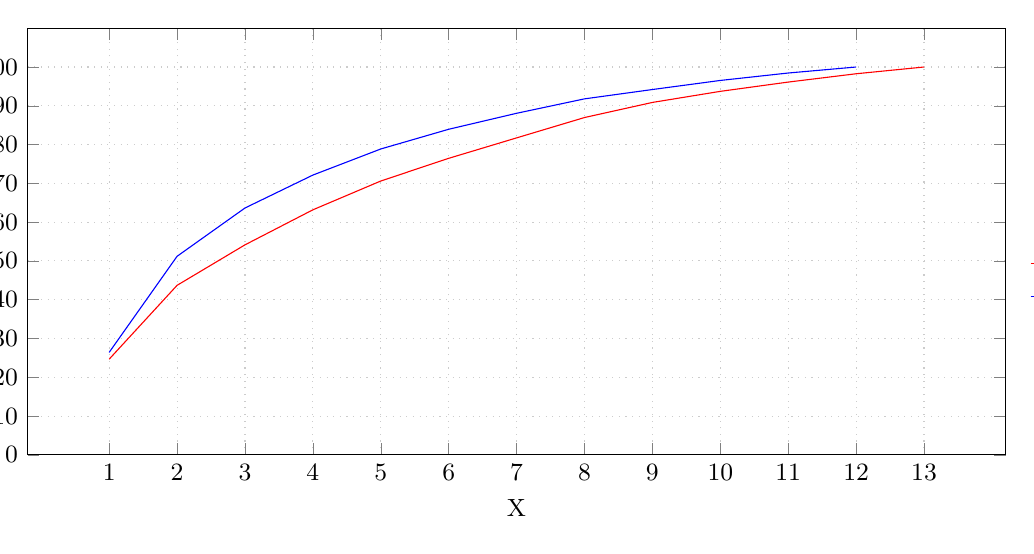
\begin{tikzpicture}[trim axis left, trim axis right]
	\begin{axis}[
		xlabel=X,
		ylabel=Y,
		xtick={1,...,13},
		ymin=0,
		ytick={0,10,...,100},
		legend style={
			at={(1,0.5)},
			xshift=0.2cm,
			anchor=north west,
			nodes=right,
			draw=none
		},
		grid=major,
   		grid style={dotted,lightgray!80!white},
		%axis lines=left
		width=14cm,
		height=7cm,
	]
	\addplot[color=red] coordinates{
		(1,24.6718)
		(2,43.7092)
		(3,54.14785132)
		(4,63.1821339)
		(5,70.60866985)
		(6,76.45681086)
		(7,81.7263871)
		(8,86.97406846)
		(9,90.86684525)
		(10,93.72329021)
		(11,96.11621437)
		(12,98.25885879)
		(13,100)		
	};
	\addplot[color=blue] coordinates{
		(1,26.42529337)
		(2,51.19458535)
		(3,63.64859236)
		(4,72.13773673)
		(5,78.8676646)
		(6,83.94694845)
		(7,88.06842906)
		(8,91.7882484)
		(9,94.19470806)
		(10,96.53607266)
		(11,98.45170481)
		(12,100)
		
	};
	\legend{Testa,Testb}
	\end{axis}
\end{tikzpicture}
\end{center}
\vspace{-3mm}
\caption{test1}
\label{fig.test1}
\vspace{3mm}
\end{figure}

\begin{figure}[ht]
\centering
\begin{tikzpicture}
\begin{axis}[
xlabel={Zeit},
ylabel={Position},
ymin=0,
ymax=6,
width=100mm,
height=80mm,
ytick={0,1,...,5},
legend style={at={(1,1)},	anchor=north east, xshift=-1mm,	yshift=-1mm}
]
\pgfplotstableread{plot/test.txt}\datatable
\addplot[color=red,mark=square*] table[x index=0,y index=1] from \datatable;
%\addplot[no markers] table[x index=0,y index=3] from \datatable;
%\addplot[no markers] table[y = Leistung] {plot/test.txt}  ;
\legend{test}
\end{axis}
\end{tikzpicture}
\caption{test2}
\label{fig.test2}
\end{figure}

\begin{figure}
\begin{center}
\begin{tikzpicture}[trim axis left, trim axis right]
  \begin{axis}[
    	ytick={0,0.1,...,1.1},
    		minor y tick num=5,
    		ymax=1.1,
    		ylabel=Y-Achse,
    		xtick={1,...,4},
    		x tick label style={align=center},
    		xticklabels={A, B},
    		boxplot/draw direction=y,
    		width=8cm,
    		height=8cm,
    		thick,
    ]
%    \addplot+[color=red,mark=x,
%    		boxplot prepared={
%      		lower whisker=,
%      		lower quartile=,
%      		median=,
%      		upper quartile=,
%      		upper whisker=
%    		},
%    ] %coordinates {};
%    table[row sep=\\,y index=0] {0.7054\\ 0.9773\\  0.9763\\ 0.9698\\ 0.7118\\ 0.6919\\ 0.9727\\ 0.7006\\ 0.974\\ 0.7077\\}; %Ausreisser
    \addplot+[color=Green,mark=x,
    		boxplot prepared={
      		median=0.3036,
      		upper quartile=0.34925,
      		lower quartile=0.2674,
      		upper whisker=0.5597,
      		lower whisker=0.18718
		},
    ] %coordinates {};
    table[row sep=\\,y index=0] {0.6045\\ 0.1818\\ 0.5826\\ 0.5688\\ 0.1814\\ 0.1825\\ 0.5750\\ 0.1783\\ 0.6312\\ 0.1793\\}; %Ausreisser
  \end{axis}
\end{tikzpicture}
\caption{Box-Whisker-Plot}
\label{fig.error_boxplot}
\end{center}
\vspace{-3mm}
\end{figure}

\subsection{Latenzzeit der Visualisierung}
Voraussetzung für die dynamische Interaktion des Benutzers mit den visualisierten Zusatzinformationen ist eine geringe Verzögerung im Visualisierungsvorgang. Nachdem die darzustellenden Bilddaten wie in \kapitel{chap.vis} beschrieben generiert wurden, werden diese über eine Ethernet-Netzwerkverbindung an das gekapselte Projektionsmodul übertragen, welches aus dem Pico-Laser-Projektor und dem Raspberry besteht.\\

\prever{
%\red[Netwerk Ethernet 10-100MBit!? Raspberry nur 10!?]\\
%\red[Raspberry pi Bezeichnung in Material]\\
}

Die Bestimmung der Latenzzeit wird mittels einer externen Kamera durchgeführt, um die Projektion und die Visualisierung innerhalb der grafischen Benutzungsschnittstelle gleichzeitig betrachten zu können. Die Kamera zeichnet die Bilddaten mit einer Frequenz $f_\ind{I}$ von \SI{50}{\Hz} auf, so dass die Dauer zwischen zwei aufgenommenen Bildern \SI{20}{\milli\second} beträgt. Dementsprechend wird auch die erreichbare Auflösung der ermittelten Latenzzeit über diese Dauer definiert. Um die Latenzzeit zu bestimmen werden die aufgezeichneten Einzelbilder ausgewertet und die Anzahl der Bilder $n_\ind{I}$ ermittelt, welche zwischen eindeutigen Abbildungen der Visualisierung liegt. Damit kann die Latenzzeit über die bekannte Aufnahmefrequenz ermittelt werden:
%
\begin{equation}
t_\ind{lat} = \frac{n_\ind{I}}{f_\ind{I}} \; \text{.}
\end{equation}

\nomenclature[l]{$t_\ind{lat}$}{Latenzzeit der Visualisierung}
\nomenclature[l]{$n_\ind{I}$}{Anzahl an aufgenommenen Bildern zwischen perspektivischer Berechnung und Visualisierung}
\nomenclature[l]{$f_\ind{I}$}{Aufnahmefrequenz der zur Bestimmung der Latenzzeit eingesetzten Kamera}

Um den Einfluss des gekapselten Projektionssystems zu bewerten wird eine Vergleichsuntersuchung durchgeführt, bei welcher die Visualisierung direkt auf dem PC erfolgt, auf welchem die weiteren Softwarekomponenten ausgeführt werden. Die durchschnittliche Latenzzeit der beiden Analysen ist zusammen mit den Leistungsdaten der Systeme in \tab{latency} aufgeführt.


%\begin{table}[ht]
%	\centering
%	\caption{Durchschnittliche Latenzzeit der Visualisierung}
%	\label{tab.latency}
%	\vspace*{-3mm}
%	\begin{tabular}[ht]{|l|r|}\hline
%		\rowcolor{Snow2}
%		System			& Durchschnittliche Latenzzeit $\bar{t}_{lat}$ [\SI{}{\milli\second}]	\\ \hline
%		Raspberry Pi 	& \SI{216}{}						\\ \hline		
%		PC				& \SI{40}{}						\\ \hline
%	\end{tabular} 
%	%\vspace*{-3mm}
%\end{table}

\begin{table}[ht]
\begin{center}
\setlength{\tabcolsep}{18pt}
\begin{tabular}{lrr}
\toprule
 & \multicolumn{1}{c}{Raspberry} & \multicolumn{1}{c}{PC}\\
\midrule
Taktfrequenz [\SI{}{\GHz}] & 0,7 & 3,2 \\ \addlinespace
Prozessor-Kerne & 1 & 4\\ \addlinespace
Arbeitsspeicher [\SI{}{GB}] & 0,5 & 8\\ \addlinespace
Durchschnittliche Latenzzeit [\SI{}{\milli\second}] & 216 & 40 \\
\bottomrule
\end{tabular}
\caption{Vergleich der Performanz von Raspberry und PC}
\label{tab.latency}
\end{center}
\end{table}

\nomenclature[a]{PC}{Personal Computer}

Die Ergebnisse zeigen, dass sich durch die Verwendung des gekapselten Projektionssystems deutliche Verzögerungen in der Visualisierung ergeben. Eine Latenzzeit von \SI{216}{\milli\second} ist für den Benutzer wahrnehmbar und kann bei der Interaktion mit den visualisierten Daten störend wirken. Die Latenzzeit der Visualisierung durch den Computer liegt hingegen bei \SI{40}{\milli\second} und sollte damit keinen merklichen Einfluss auf die Dynamik der Interaktion haben. Der ermittelte Unterschied in den Latenzzeiten ergibt sich dabei aus der Kombination von höherer Rechenleistung des Computers und der  durch die Netzwerkverbindung hervorgerufenen Verzögerung.\\

Ein Grund für die Ausgliederung des Projektionsvorgangs mittels des Raspberry lag darin, ein Projektionsmodul zum Einsatz in ROS basierten Anwendungen zur Verfügung zu stellen. Die Rechenkapazität des Raspberry sollte genutzt werden, um die verfügbaren Ressourcen des verwendeten Computers auf die anderen Softwaremodule aufzuteilen. Im Zusammenhang mit der entwickelten Anwendung für das \kps{} sind die zusätzlichen Rechenressourcen gegenüber der Dynamik der Interaktion abzuwägen. In Anwendungsfällen, in denen ausreichend Rechenkapazität zur Verfügung steht, sollte daher unter Umständen auf die Auslagerung der Projektion verzichtet werden.